%%%%%%%%%%%%%
%Coverage plots
%Identity figures, uncomment
\begin{figure}[!hbtp]
  \centering
  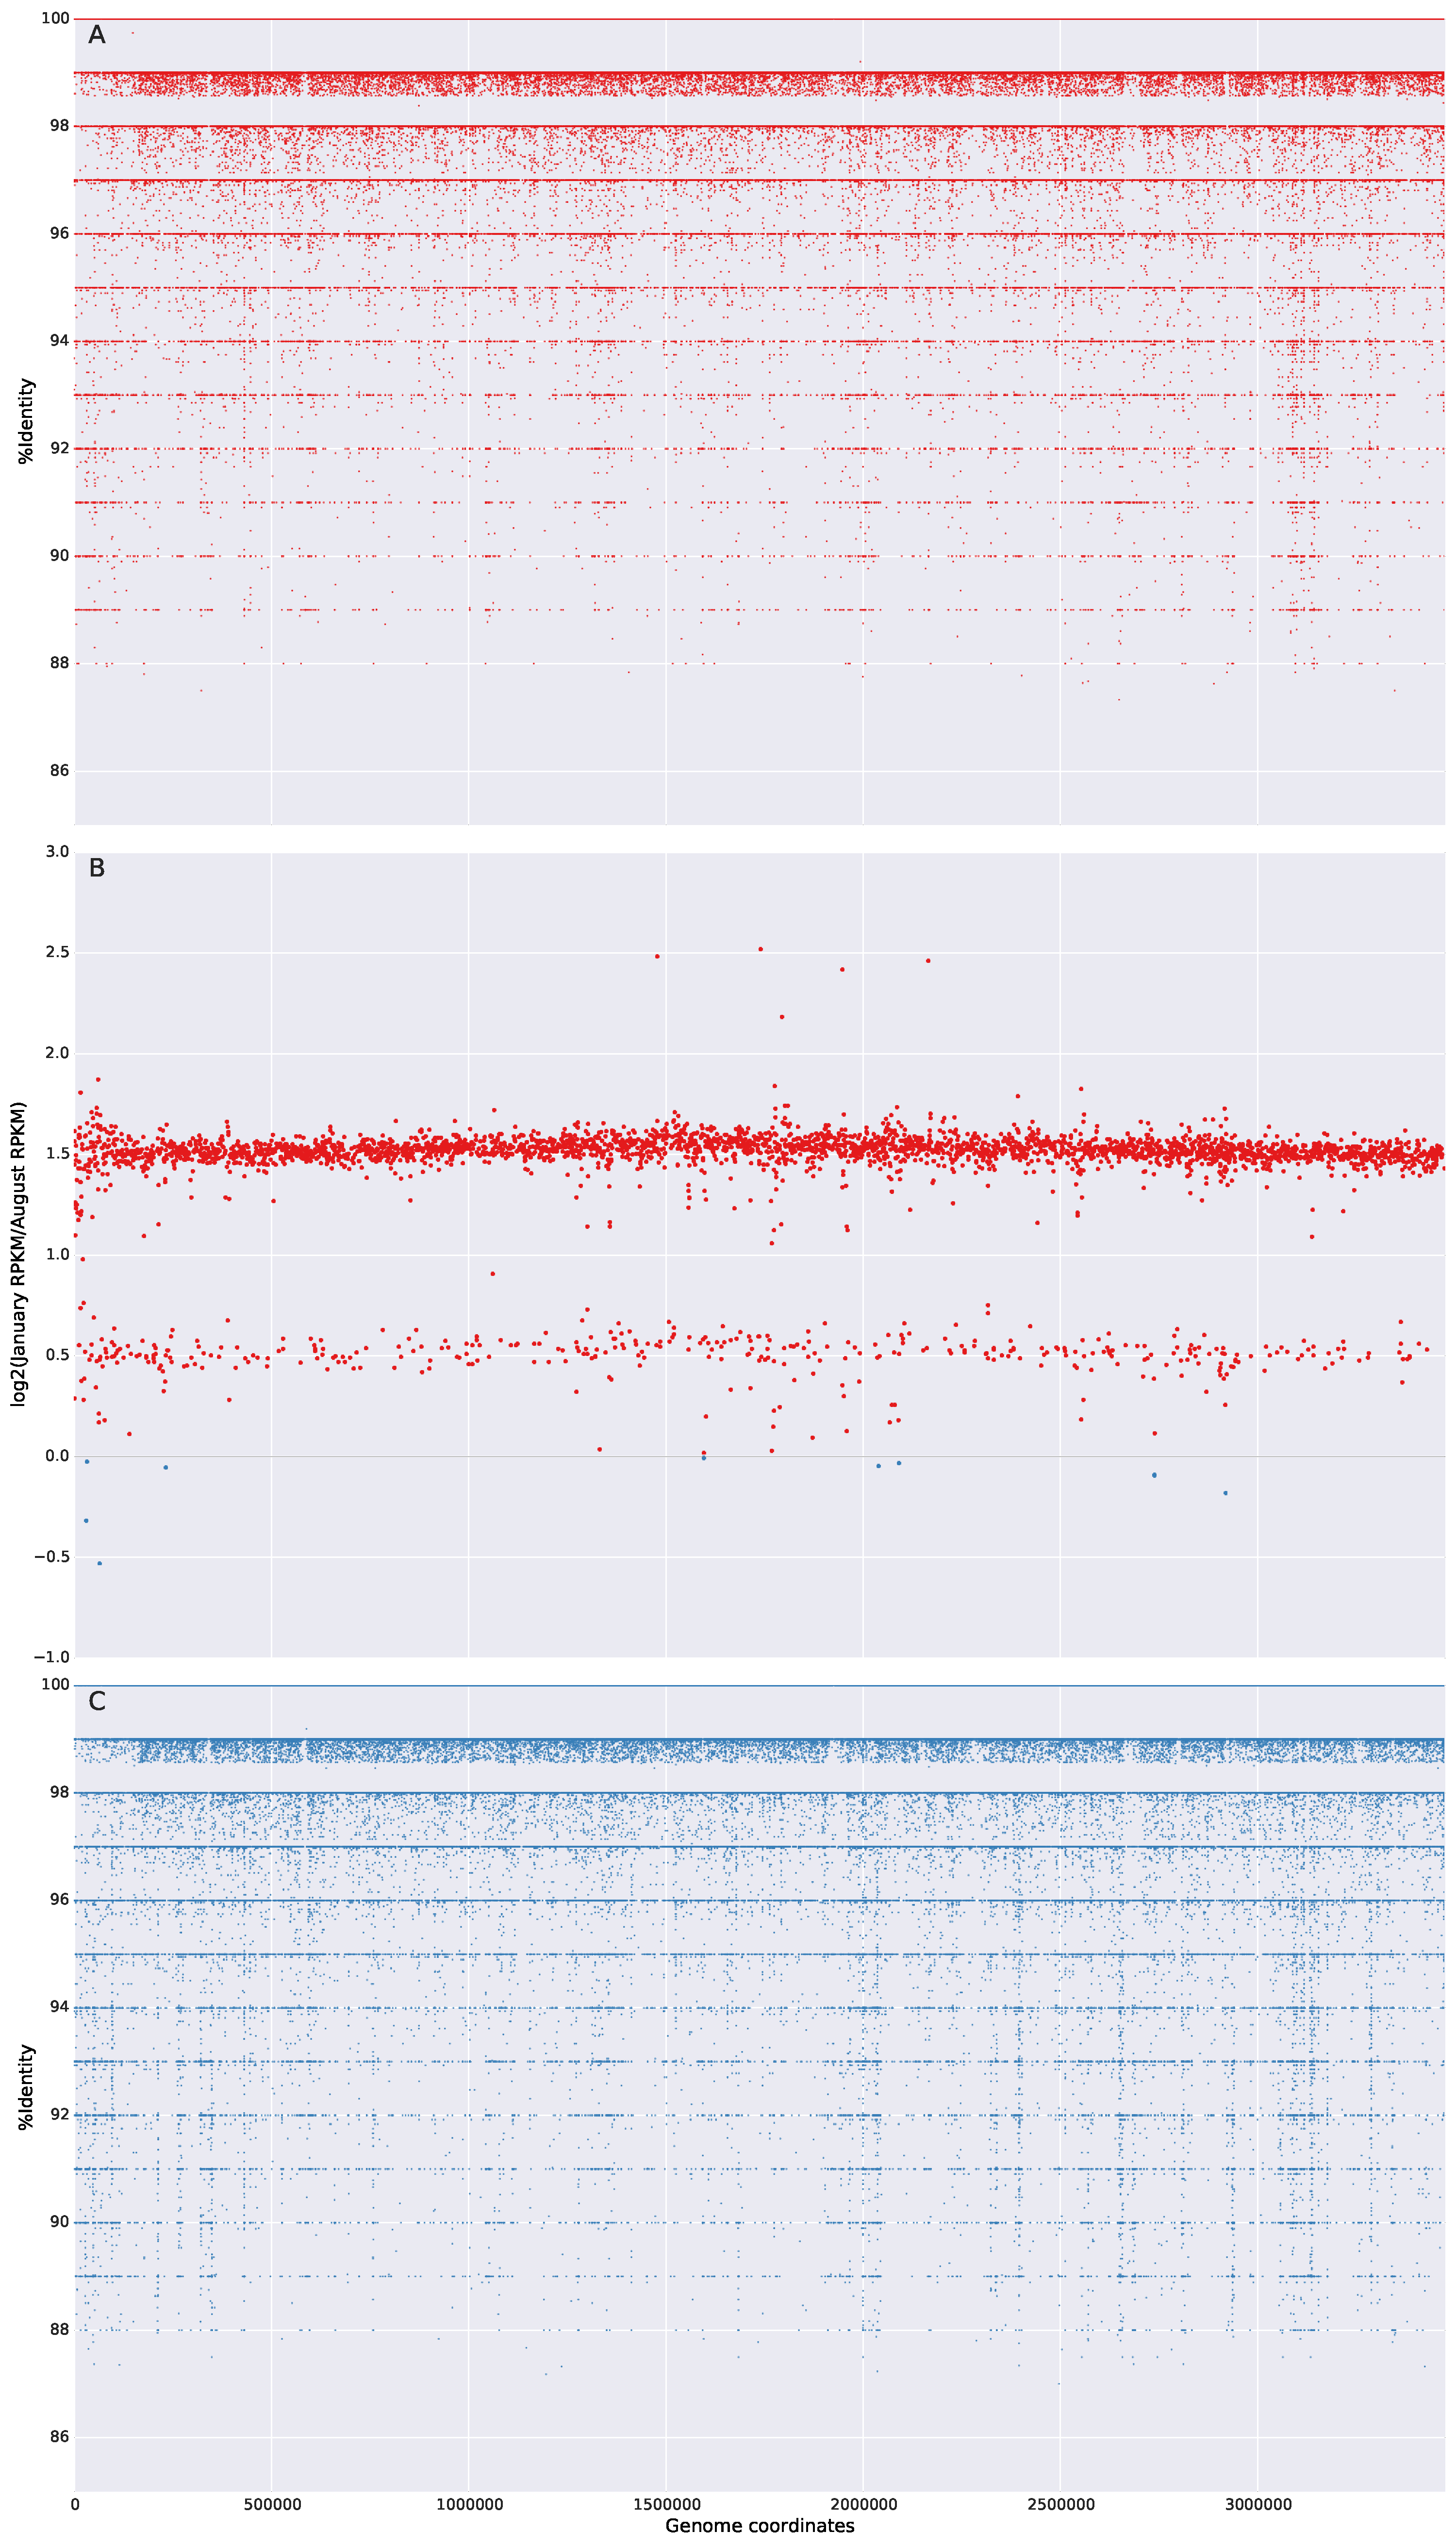
\includegraphics[width=\textwidth,height=\textheight,keepaspectratio]{Chapter5/Figures/coverage_plots/J07HWQ1_coverage.pdf}
  \caption{J07HWQ1coverage}
  \label{J07HWQ1coverage}
\end{figure}

\begin{figure}[!hbtp]
  \centering
  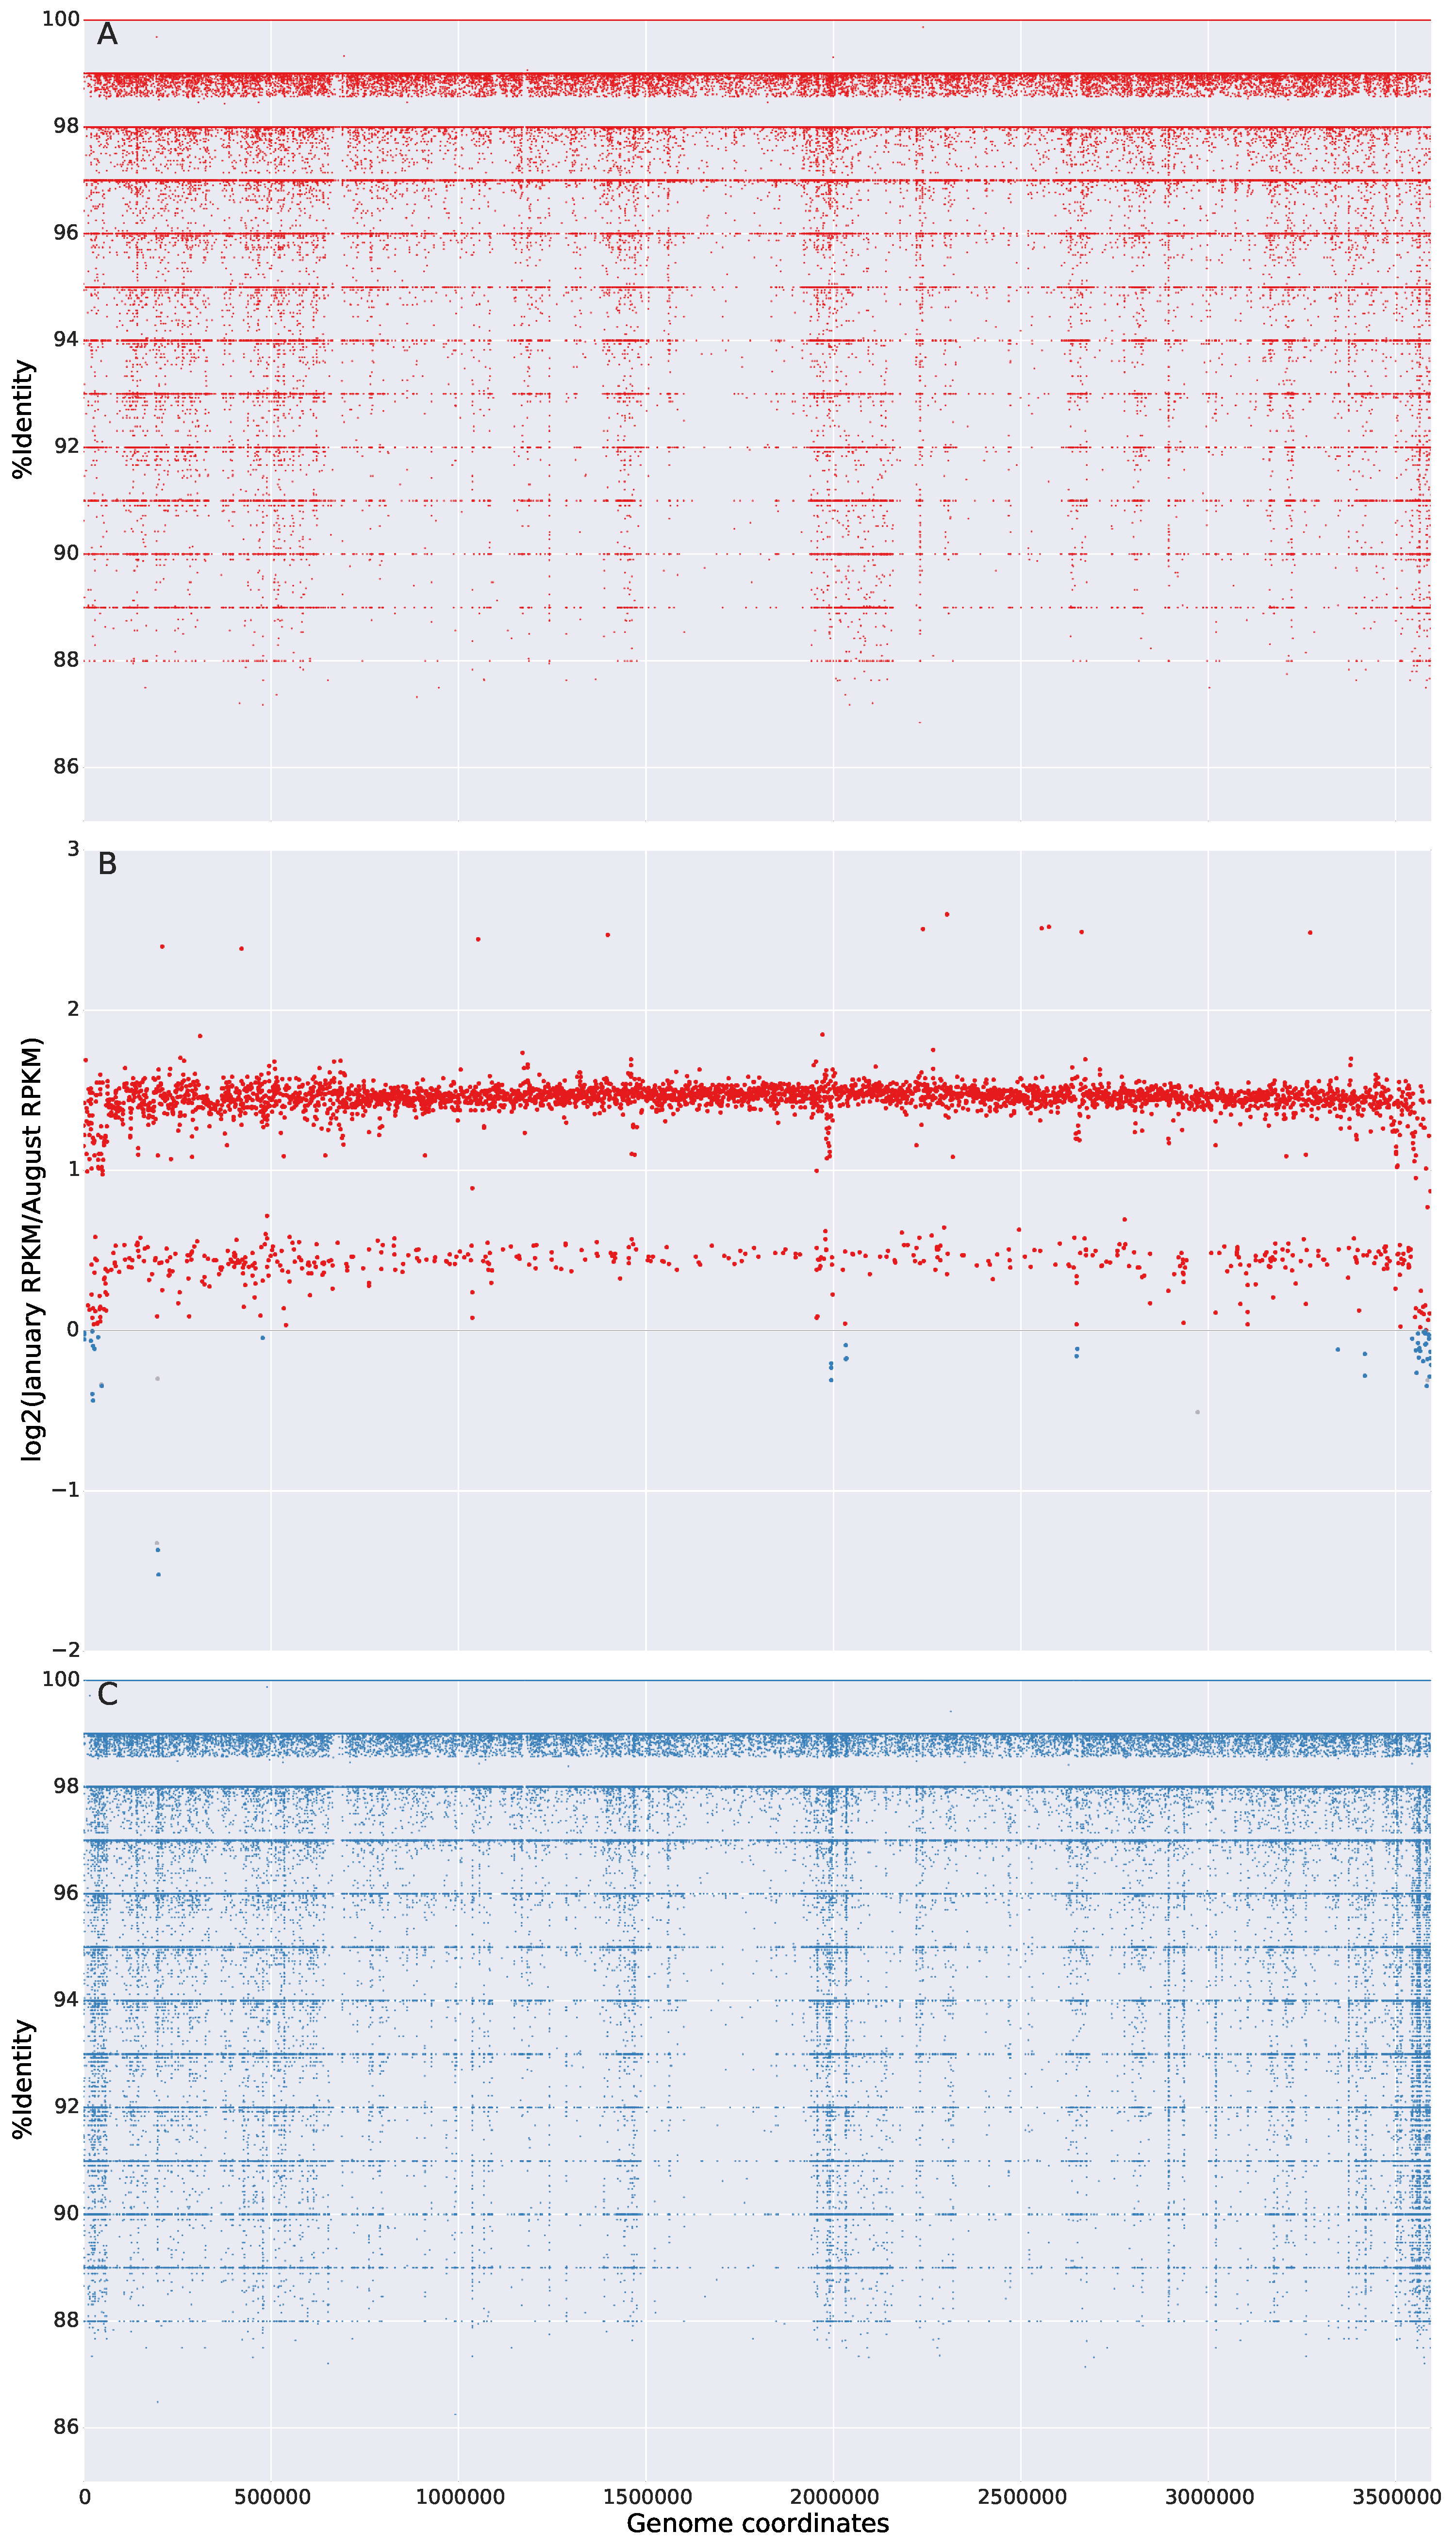
\includegraphics[width=\textwidth,height=\textheight,keepaspectratio]{Chapter5/Figures/coverage_plots/J07HWQ2_coverage.pdf}
  \caption{J07HWQ2coverage}
  \label{J07HWQ2coverage}
\end{figure}

\begin{figure}[!hbtp]
  \centering
  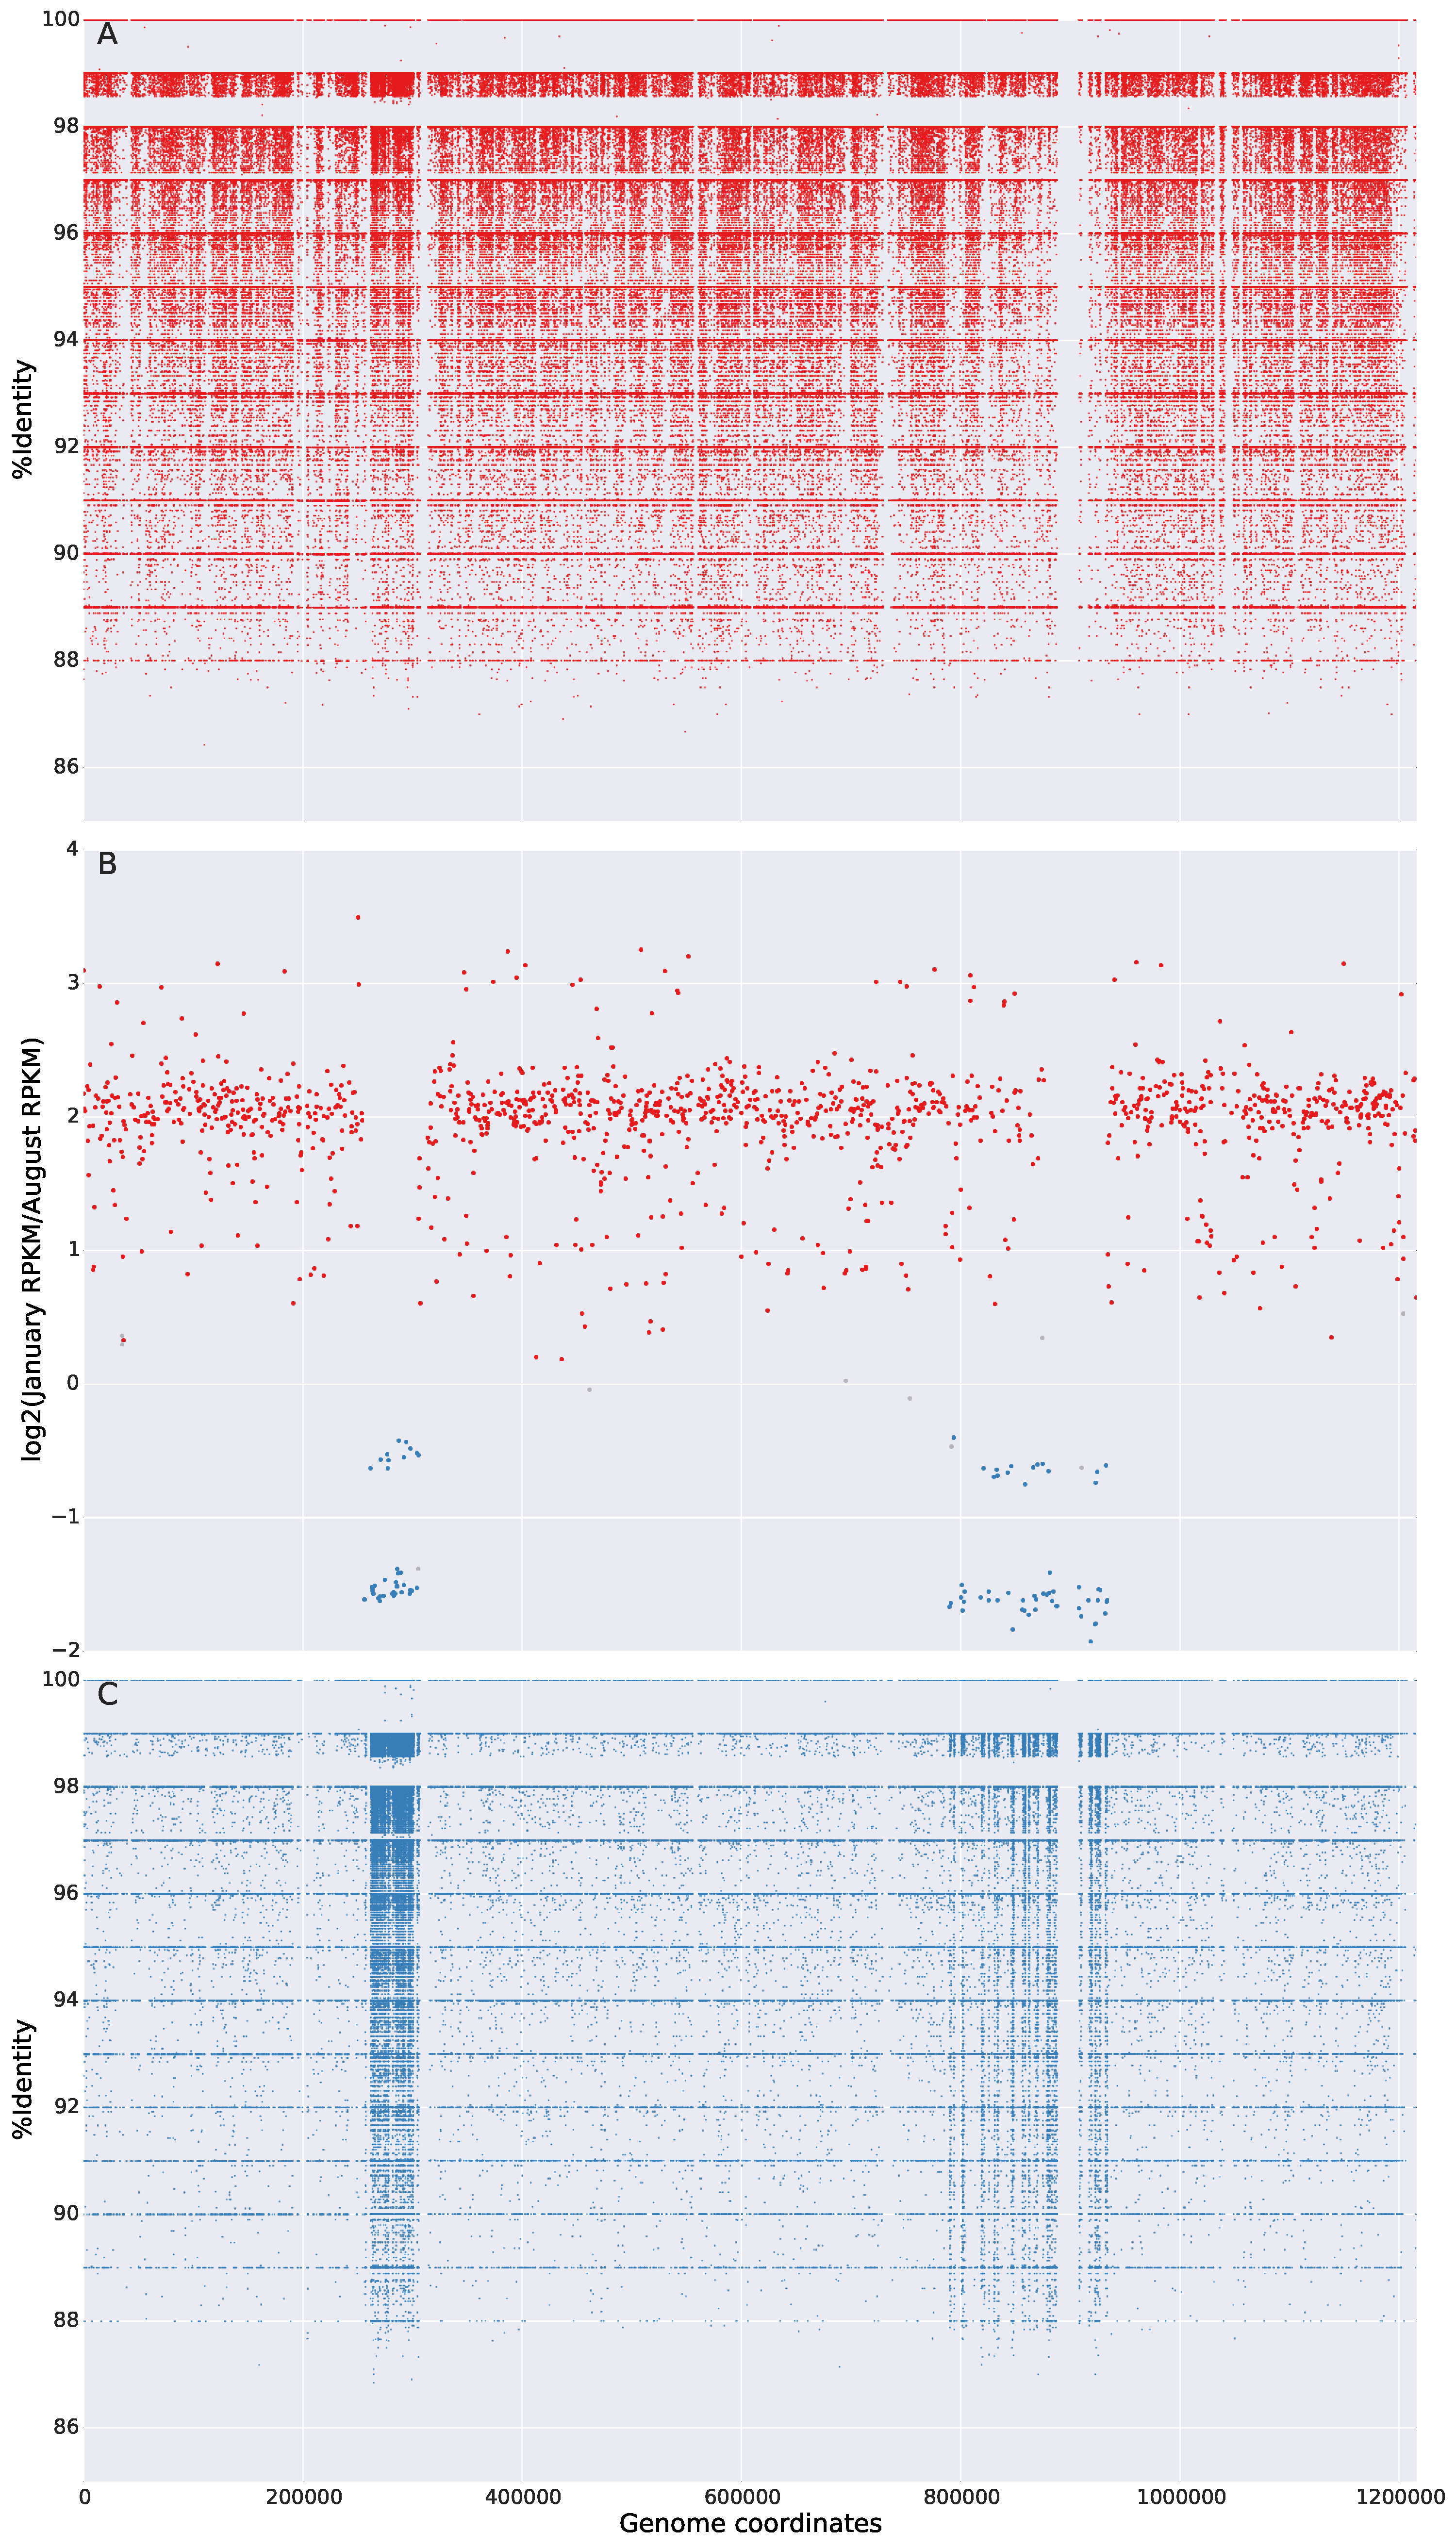
\includegraphics[width=\textwidth,height=\textheight,keepaspectratio]{Chapter5/Figures/coverage_plots/J07AB56_coverage.pdf}
  \caption{J07AB56coverage}
  \label{J07AB56coverage}
\end{figure}

\begin{figure}[!hbtp]
  \centering
  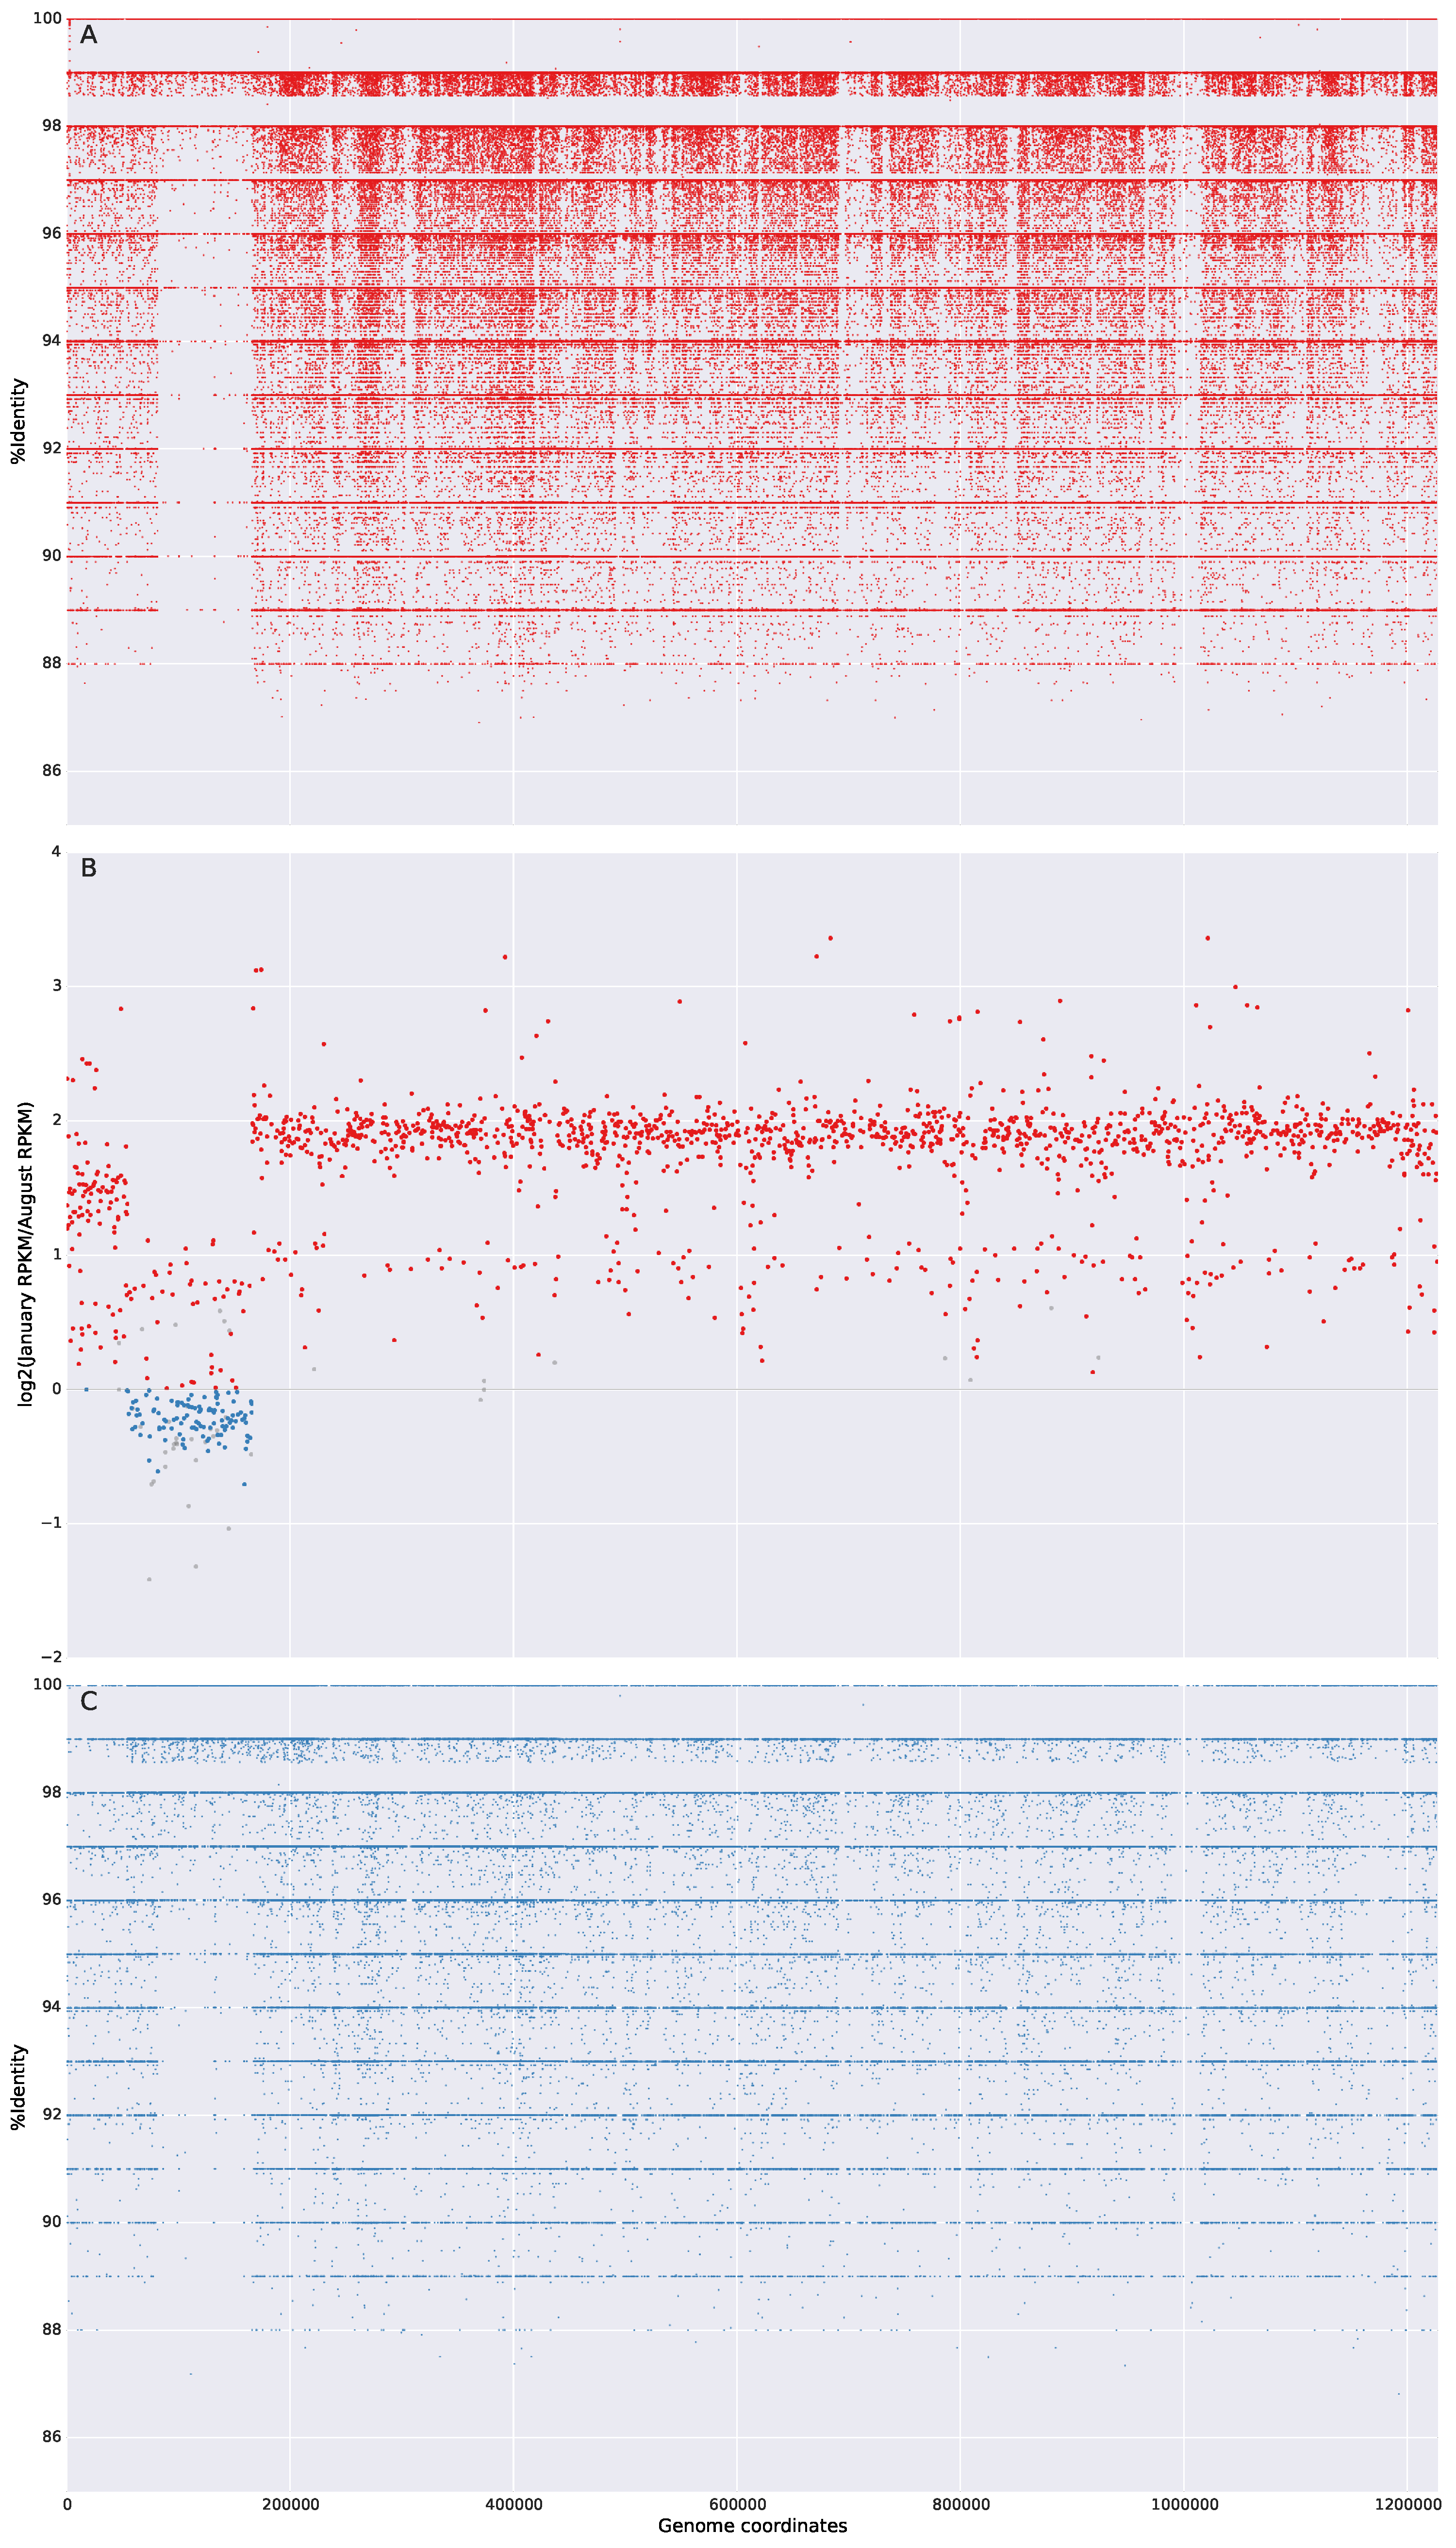
\includegraphics[width=\textwidth,height=\textheight,keepaspectratio]{Chapter5/Figures/coverage_plots/J07AB43_coverage.pdf}
  \caption{J07AB43coverage}
  \label{J07AB43ccoverage}
\end{figure}

\begin{figure}[!hbtp]
  \centering
  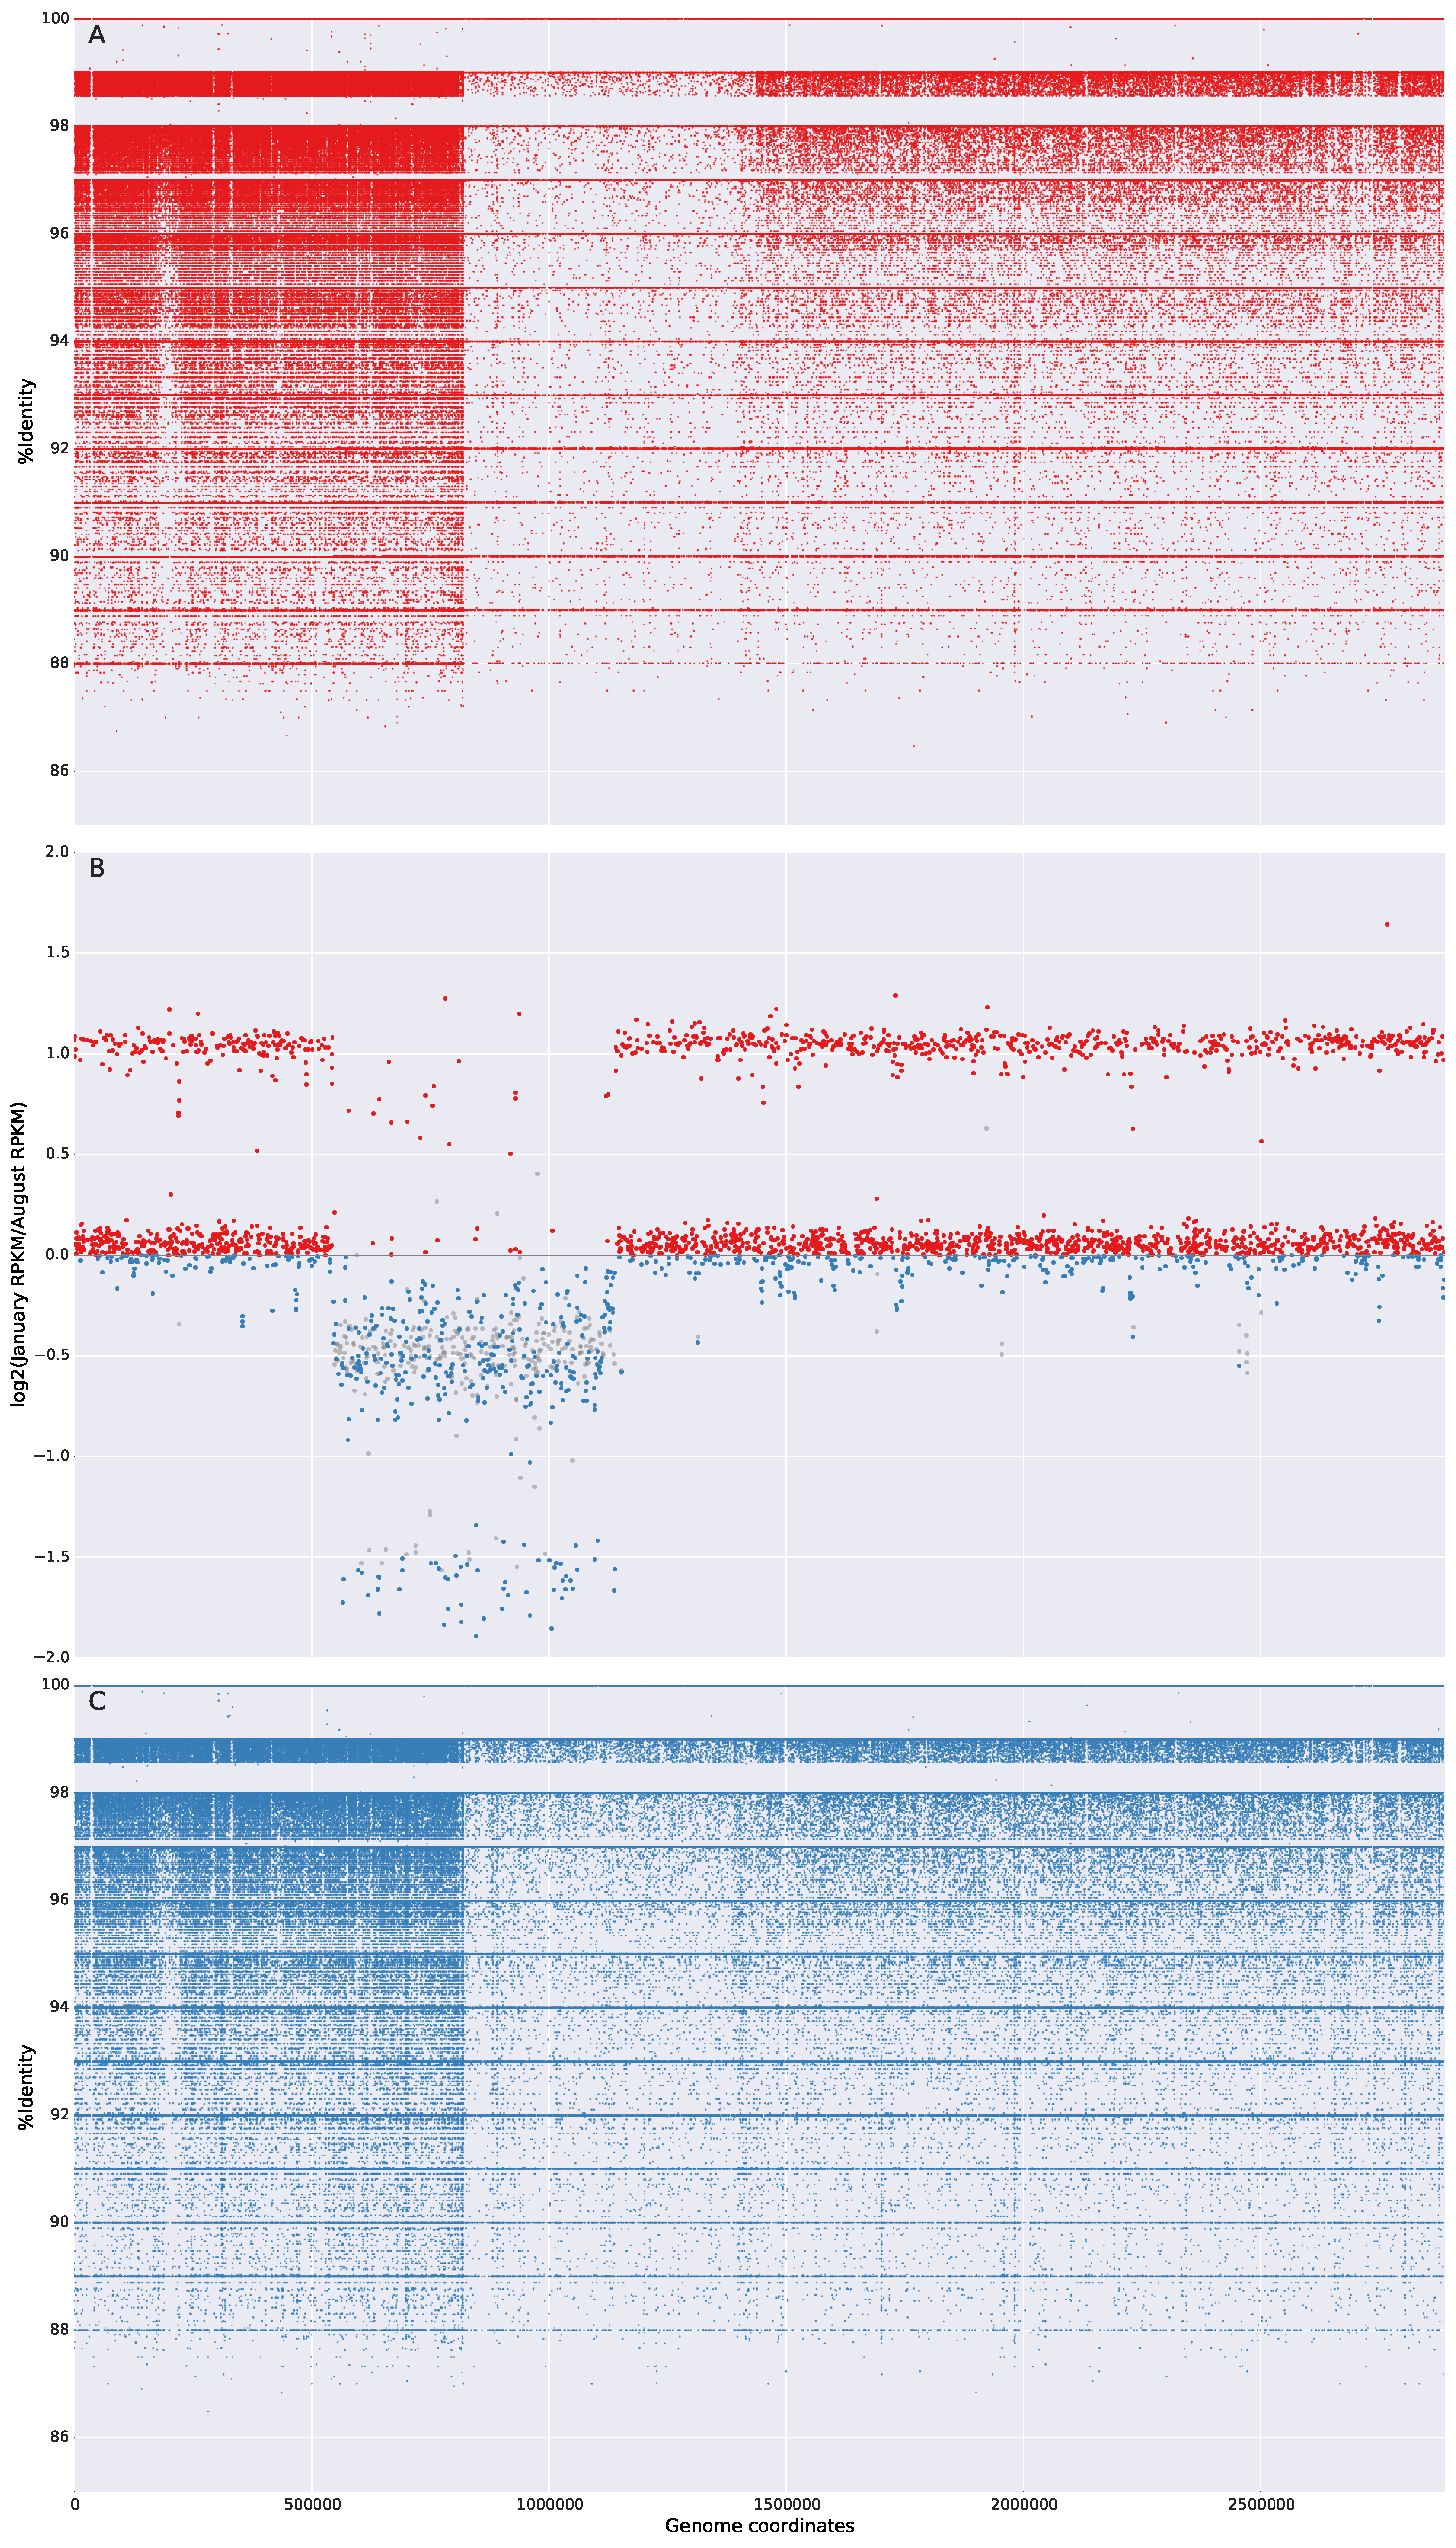
\includegraphics[width=\textwidth,height=\textheight,keepaspectratio]{Chapter5/Figures/coverage_plots/J07HN4_coverage.pdf}
  \caption{J07HN4coverage}
  \label{J07HN4coverage}
\end{figure}

\begin{figure}[!hbtp]
  \centering
  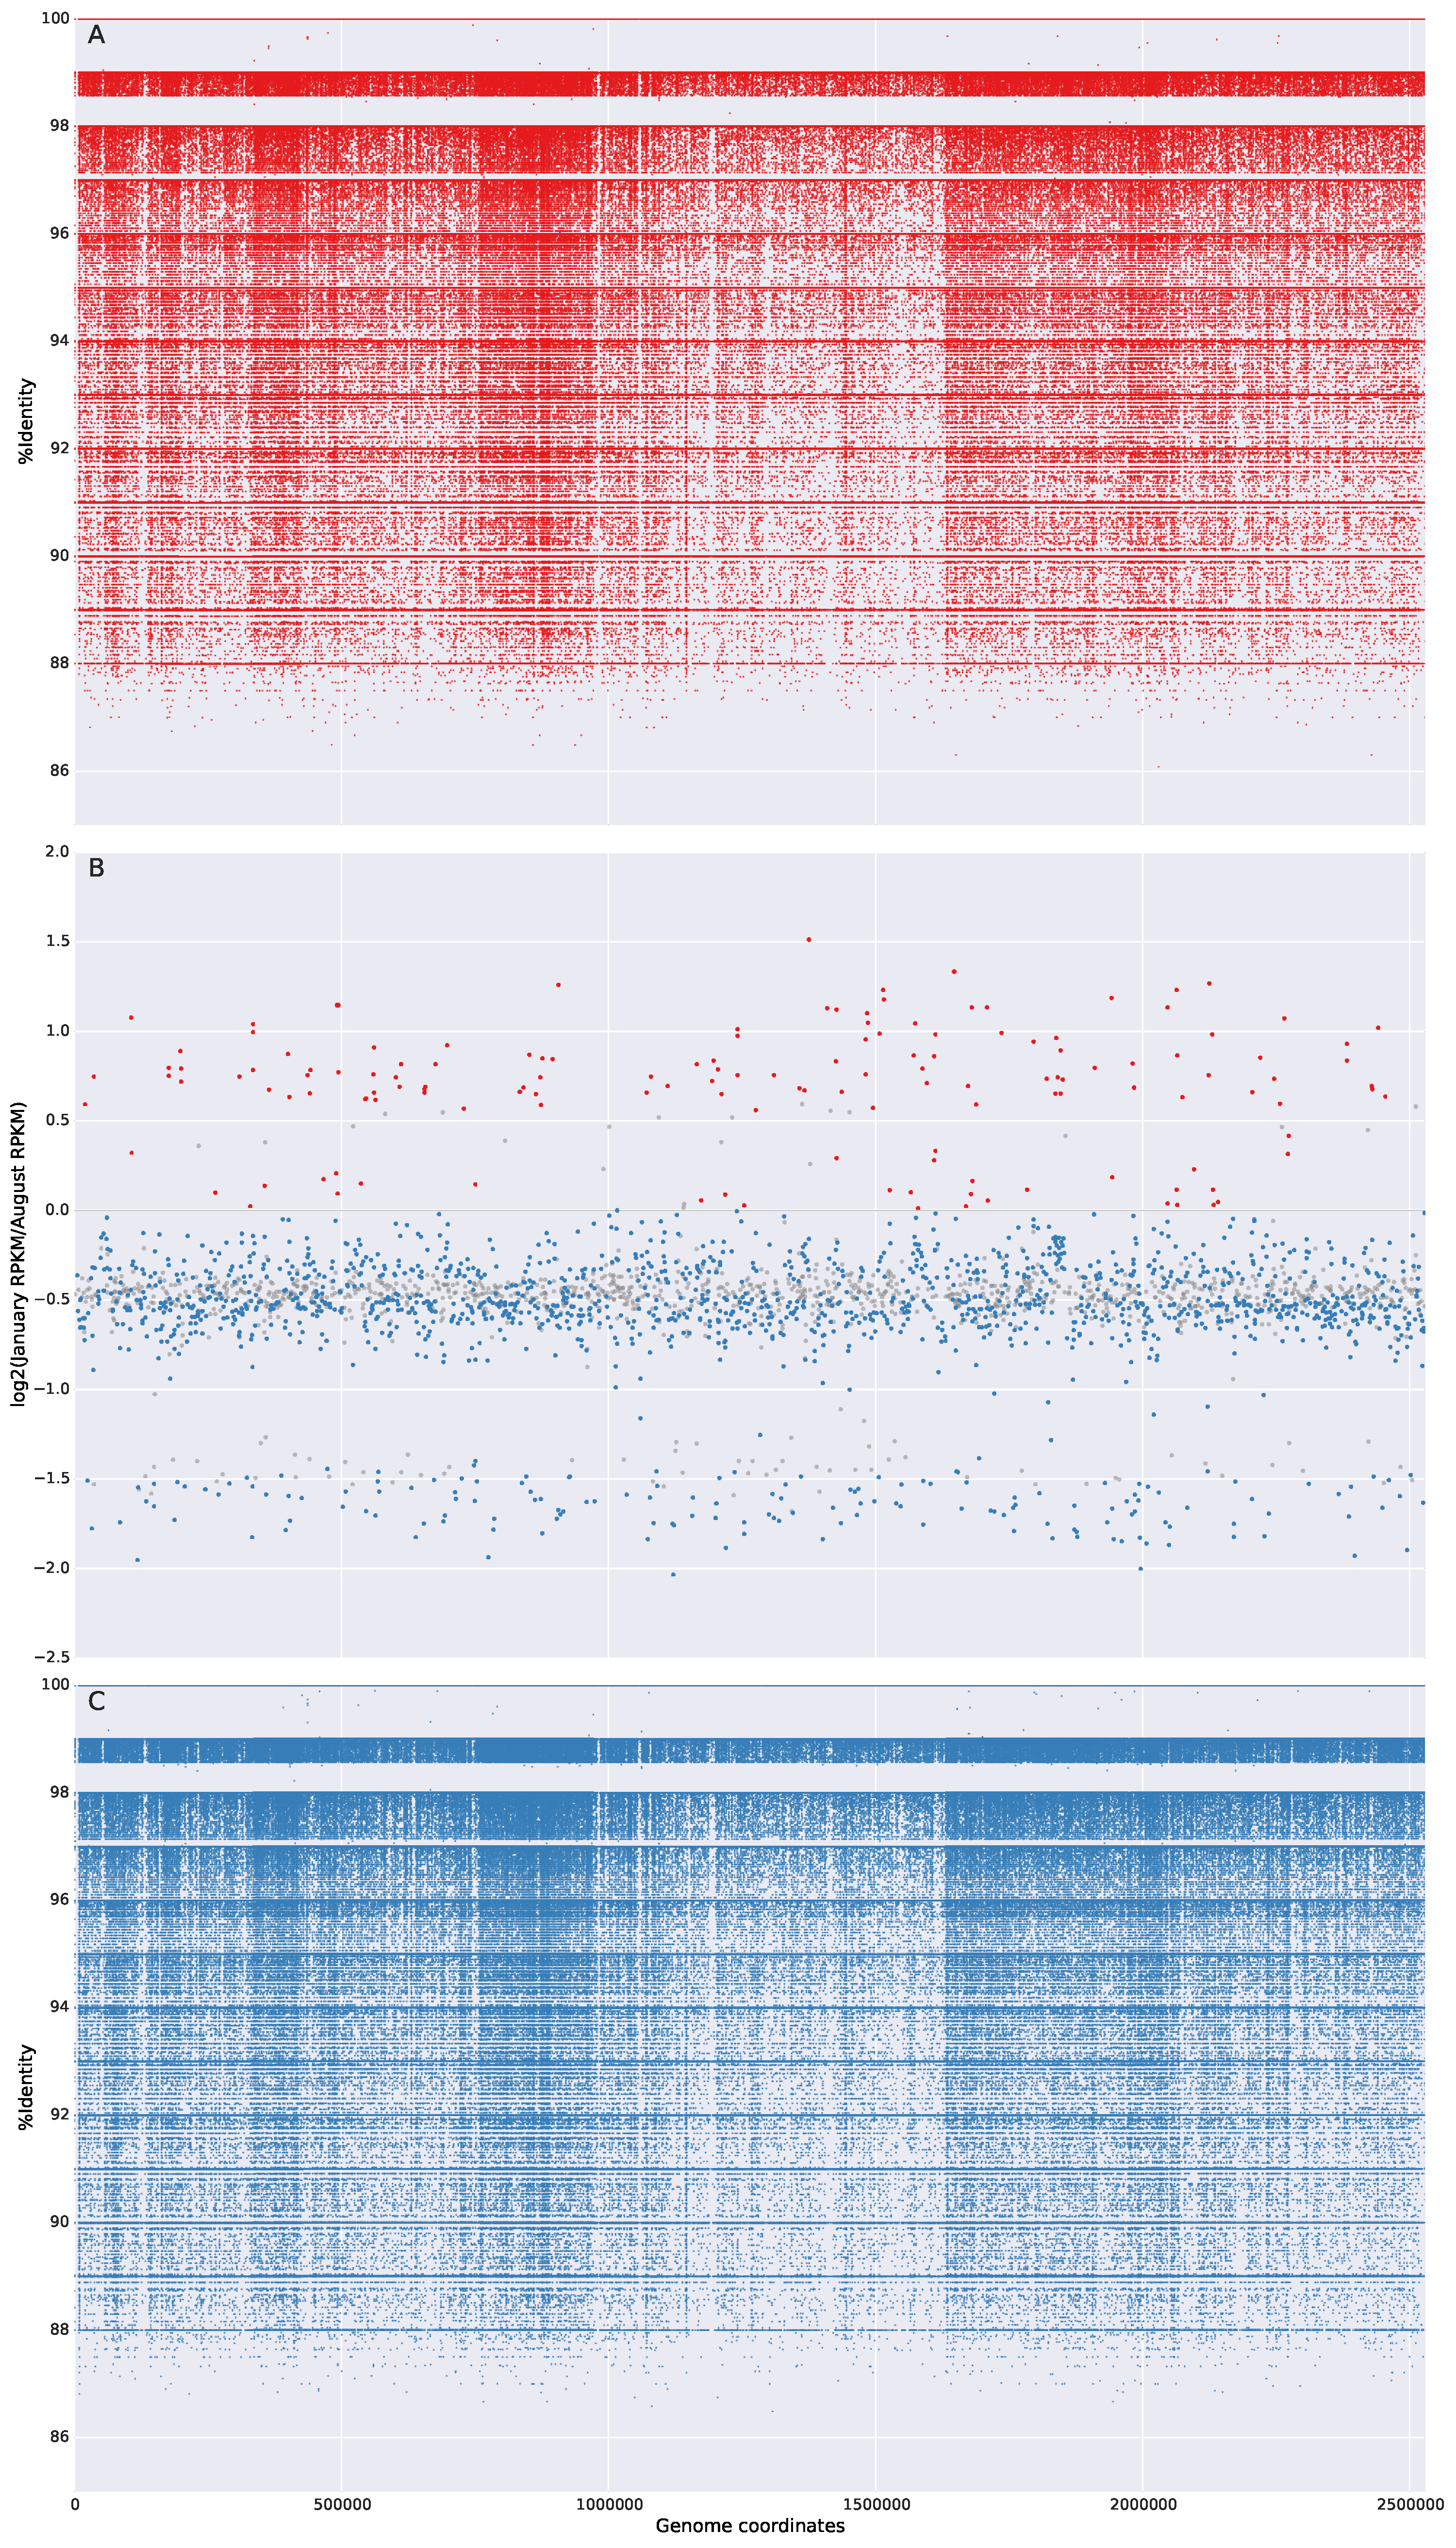
\includegraphics[width=\textwidth,height=\textheight,keepaspectratio]{Chapter5/Figures/coverage_plots/J07HN6_coverage.pdf}
  \caption{J07HN6coverage}
  \label{J07HN6coverage}
\end{figure}

\begin{figure}[!hbtp]
  \centering
  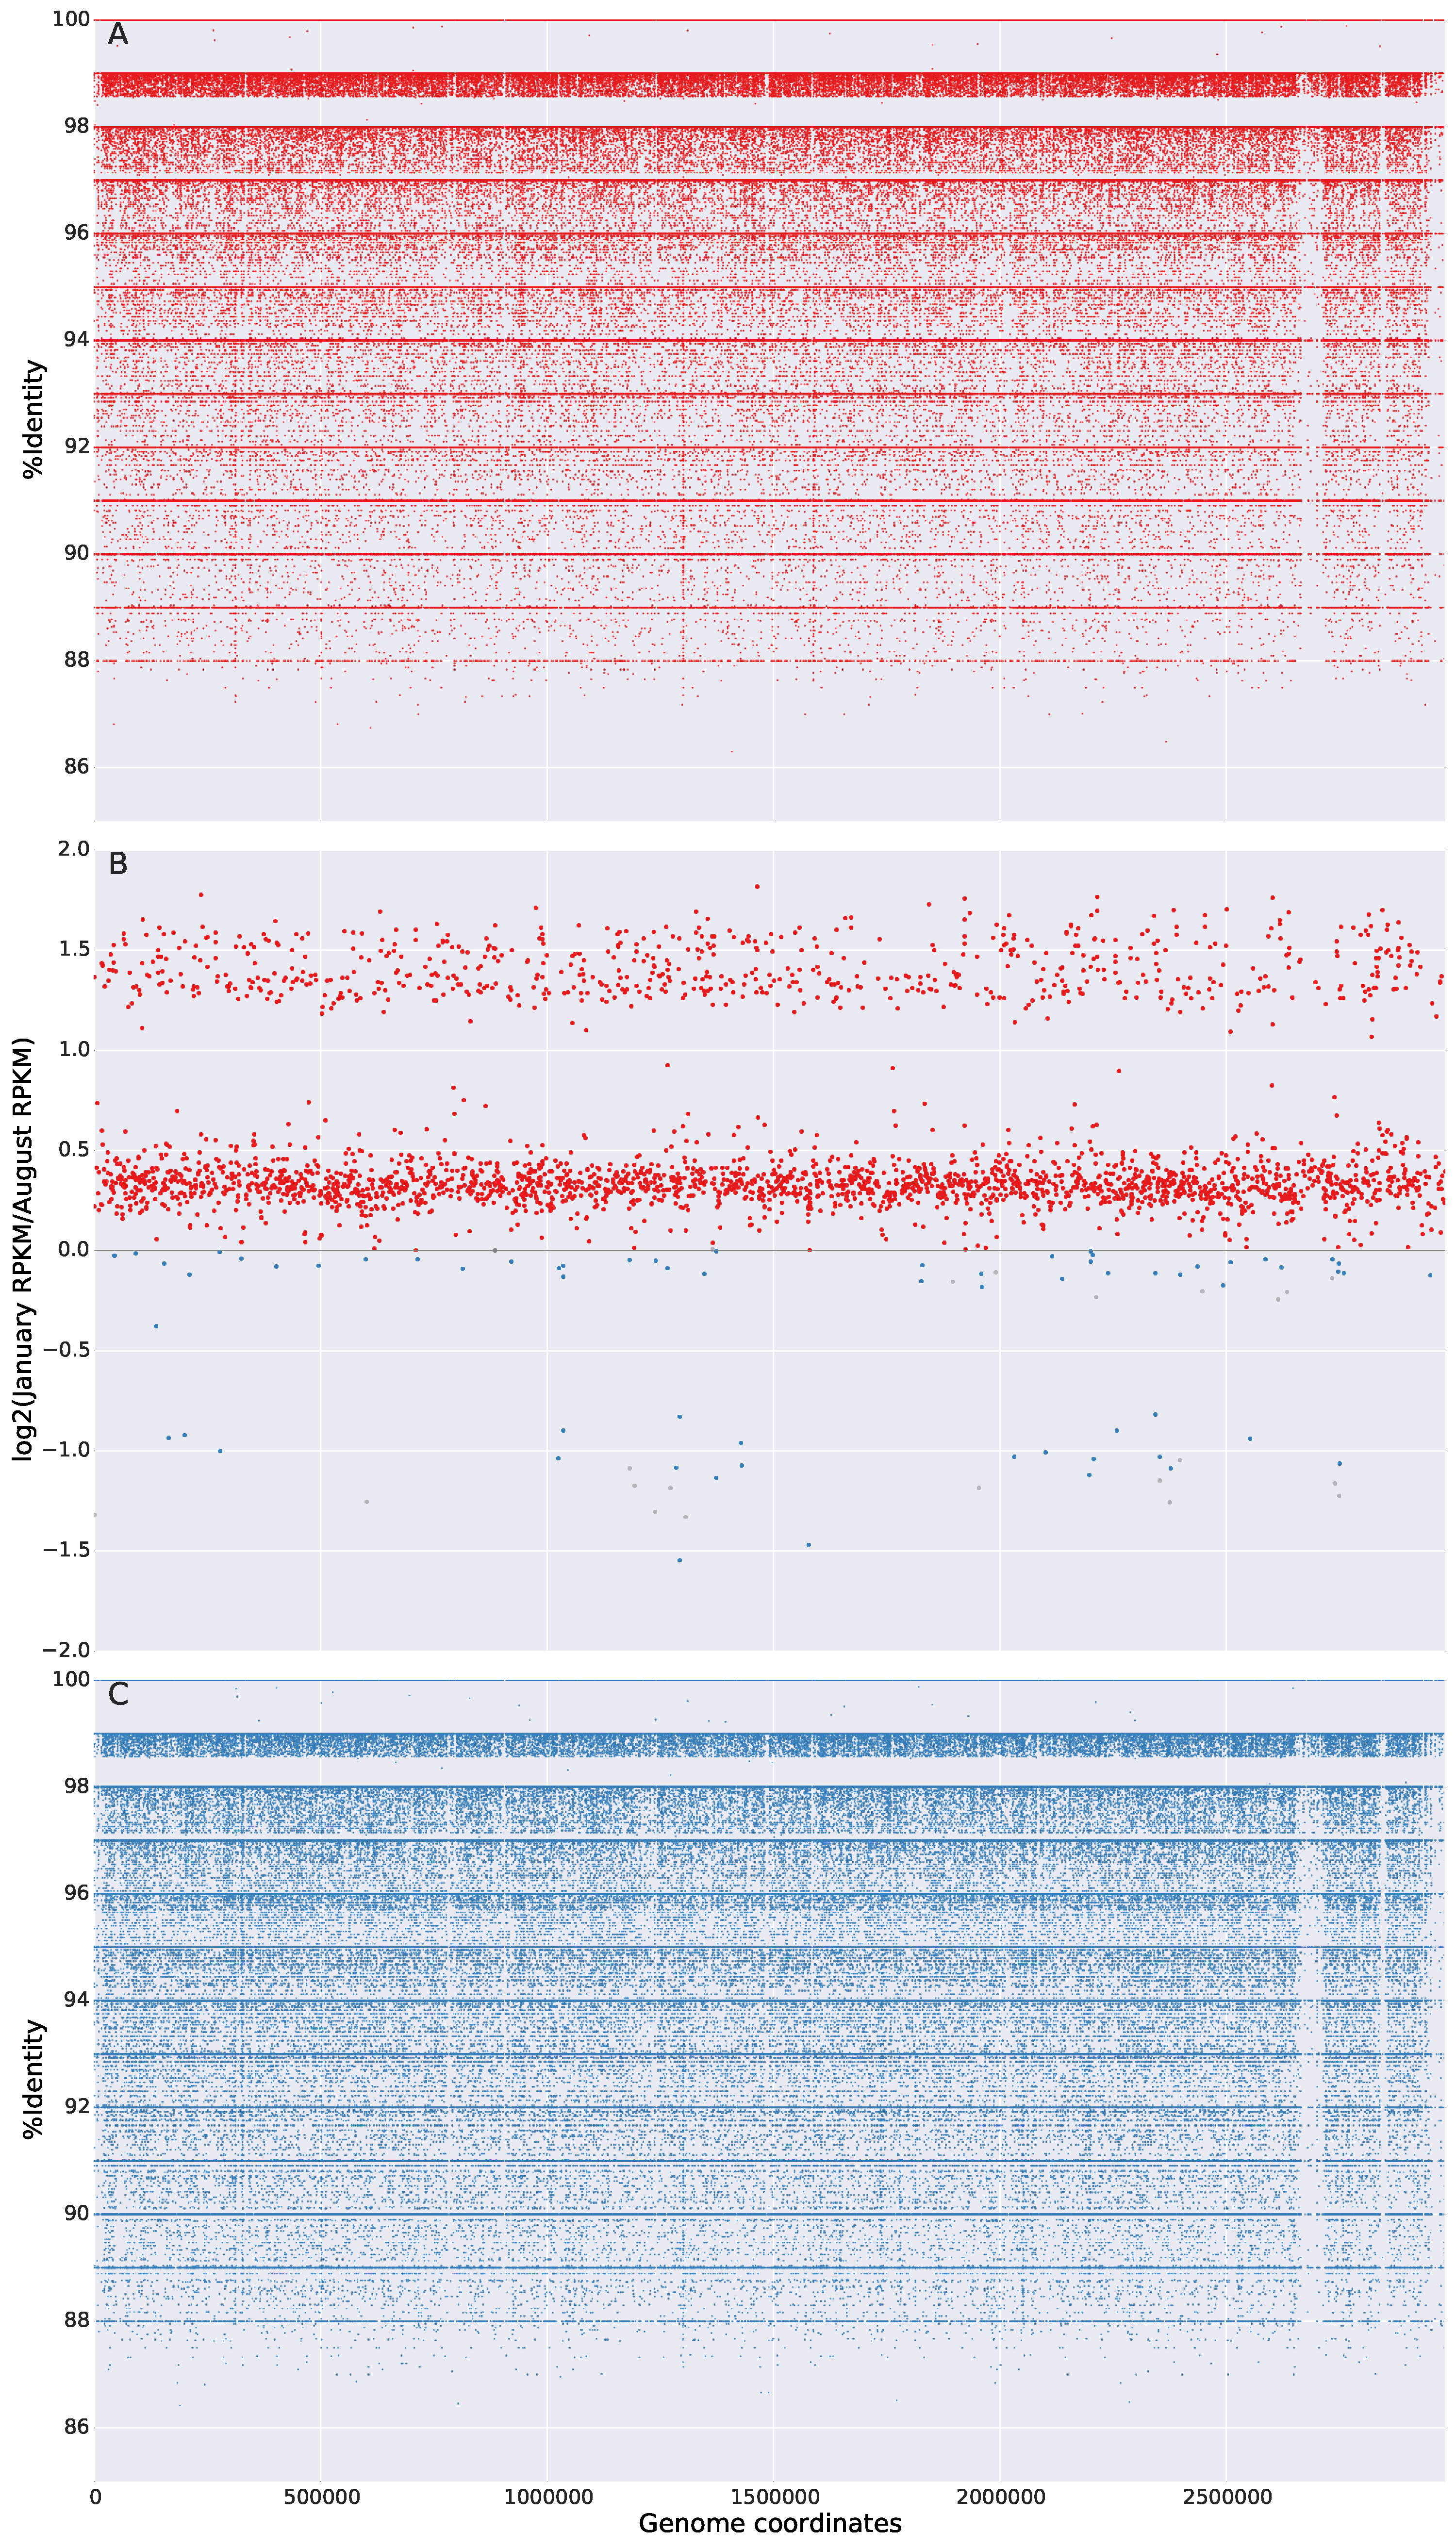
\includegraphics[width=\textwidth,height=\textheight,keepaspectratio]{Chapter5/Figures/coverage_plots/J07HX64_coverage.pdf}
  \caption{J07HN64coverage}
  \label{J07HN64coverage}
\end{figure}

\begin{figure}[!hbtp]
  \centering
  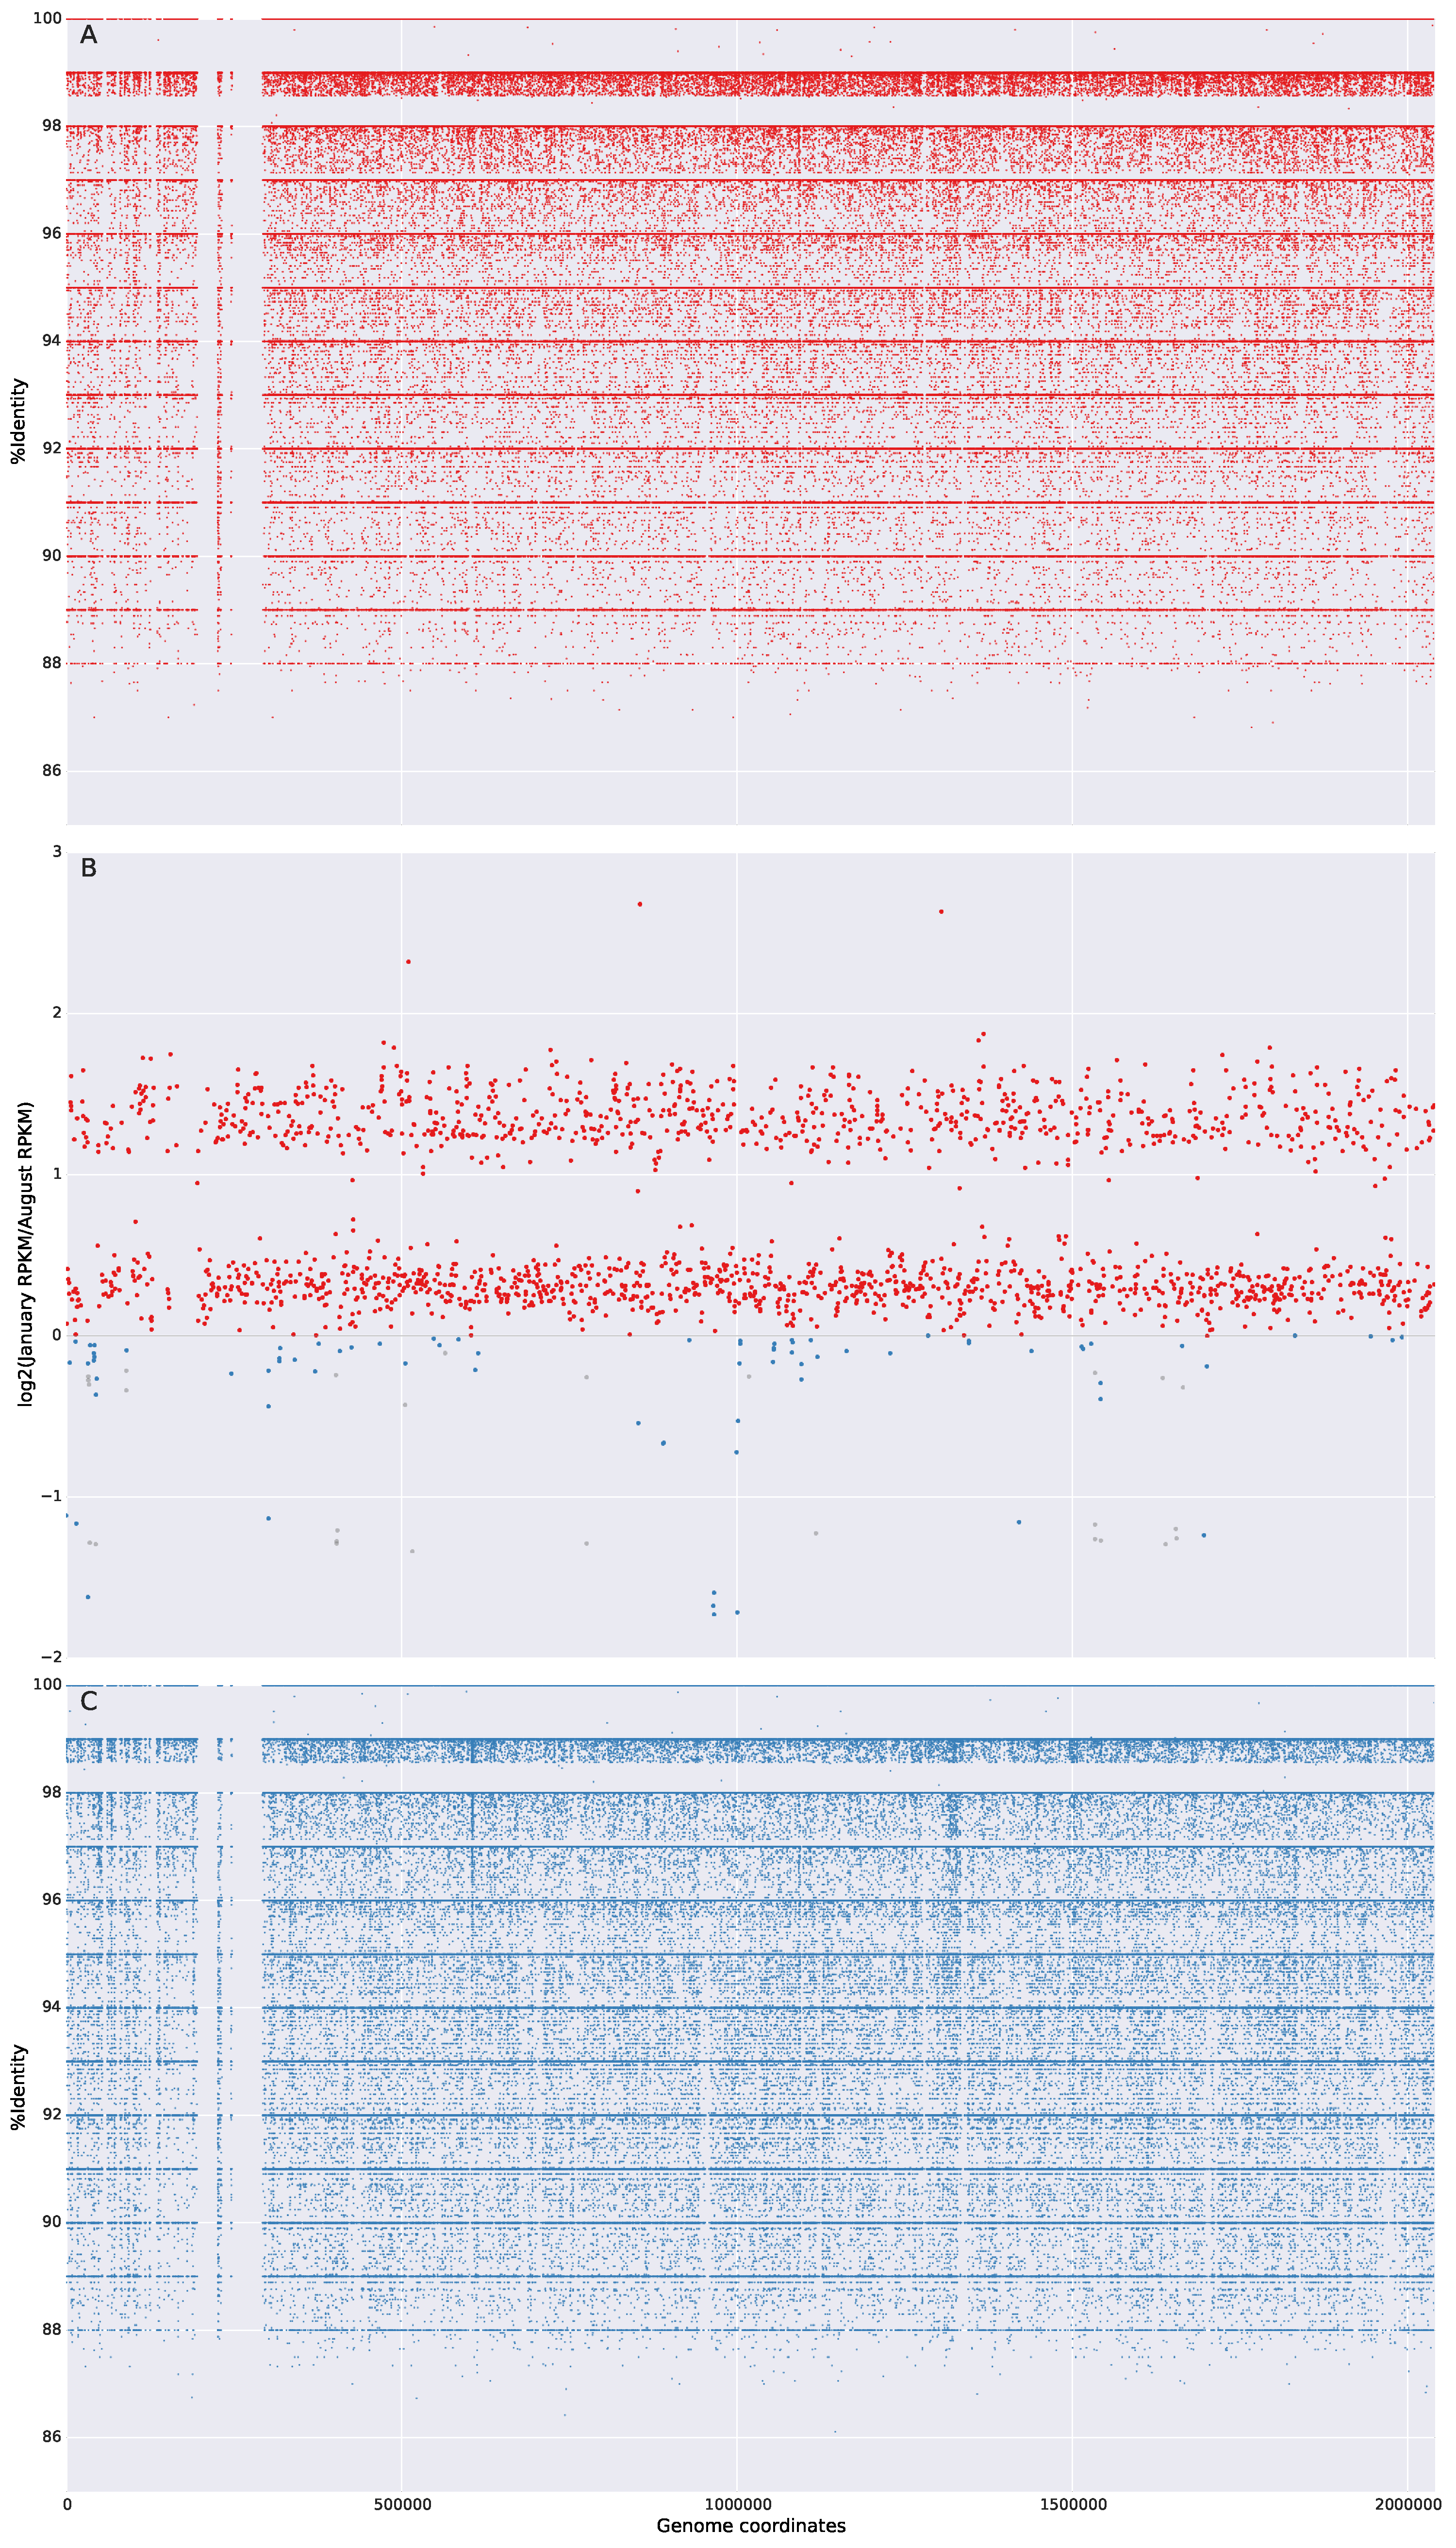
\includegraphics[width=\textwidth,height=\textheight,keepaspectratio]{Chapter5/Figures/coverage_plots/J07HX5_coverage.pdf}
  \caption{J07HX5coverage}
  \label{J07HX5coverage}
\end{figure}

\begin{figure}[!hbtp]
  \centering
  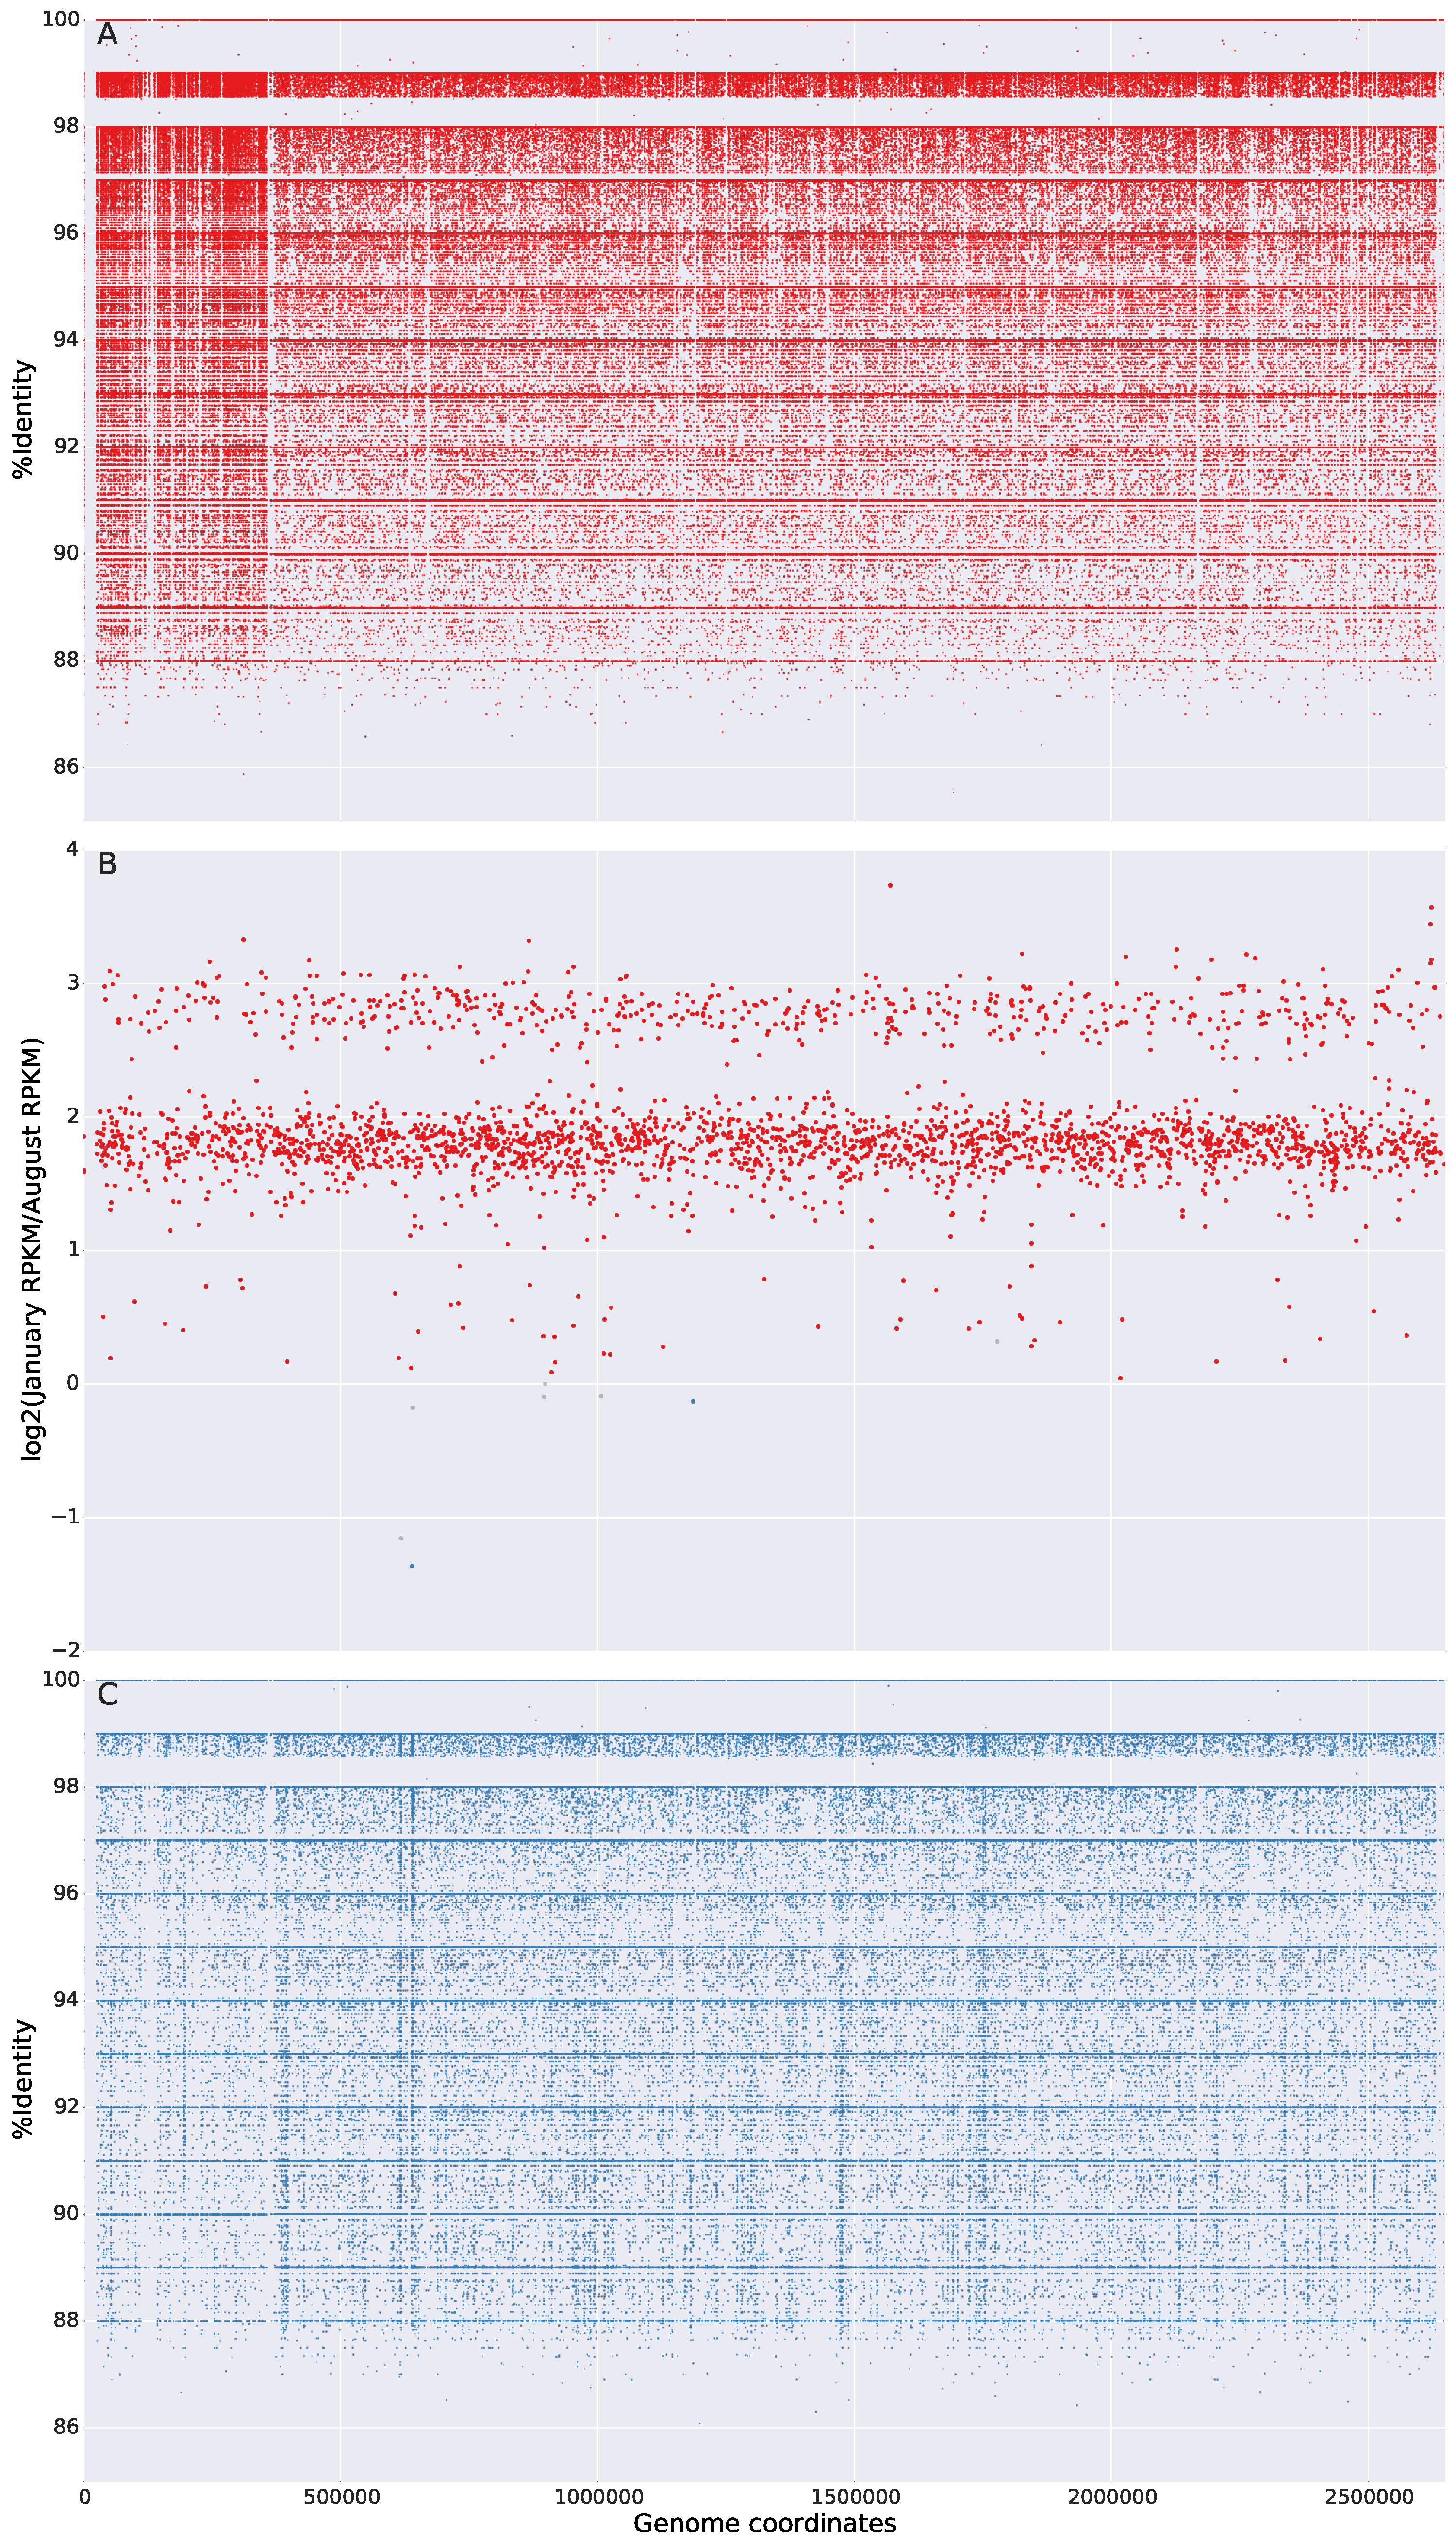
\includegraphics[width=\textwidth,height=\textheight,keepaspectratio]{Chapter5/Figures/coverage_plots/J07HB67_coverage.pdf}
  \caption{J07HB67coverage}
  \label{J07HB67coverage}
\end{figure}

\begin{figure}[!hbtp]
  \centering
  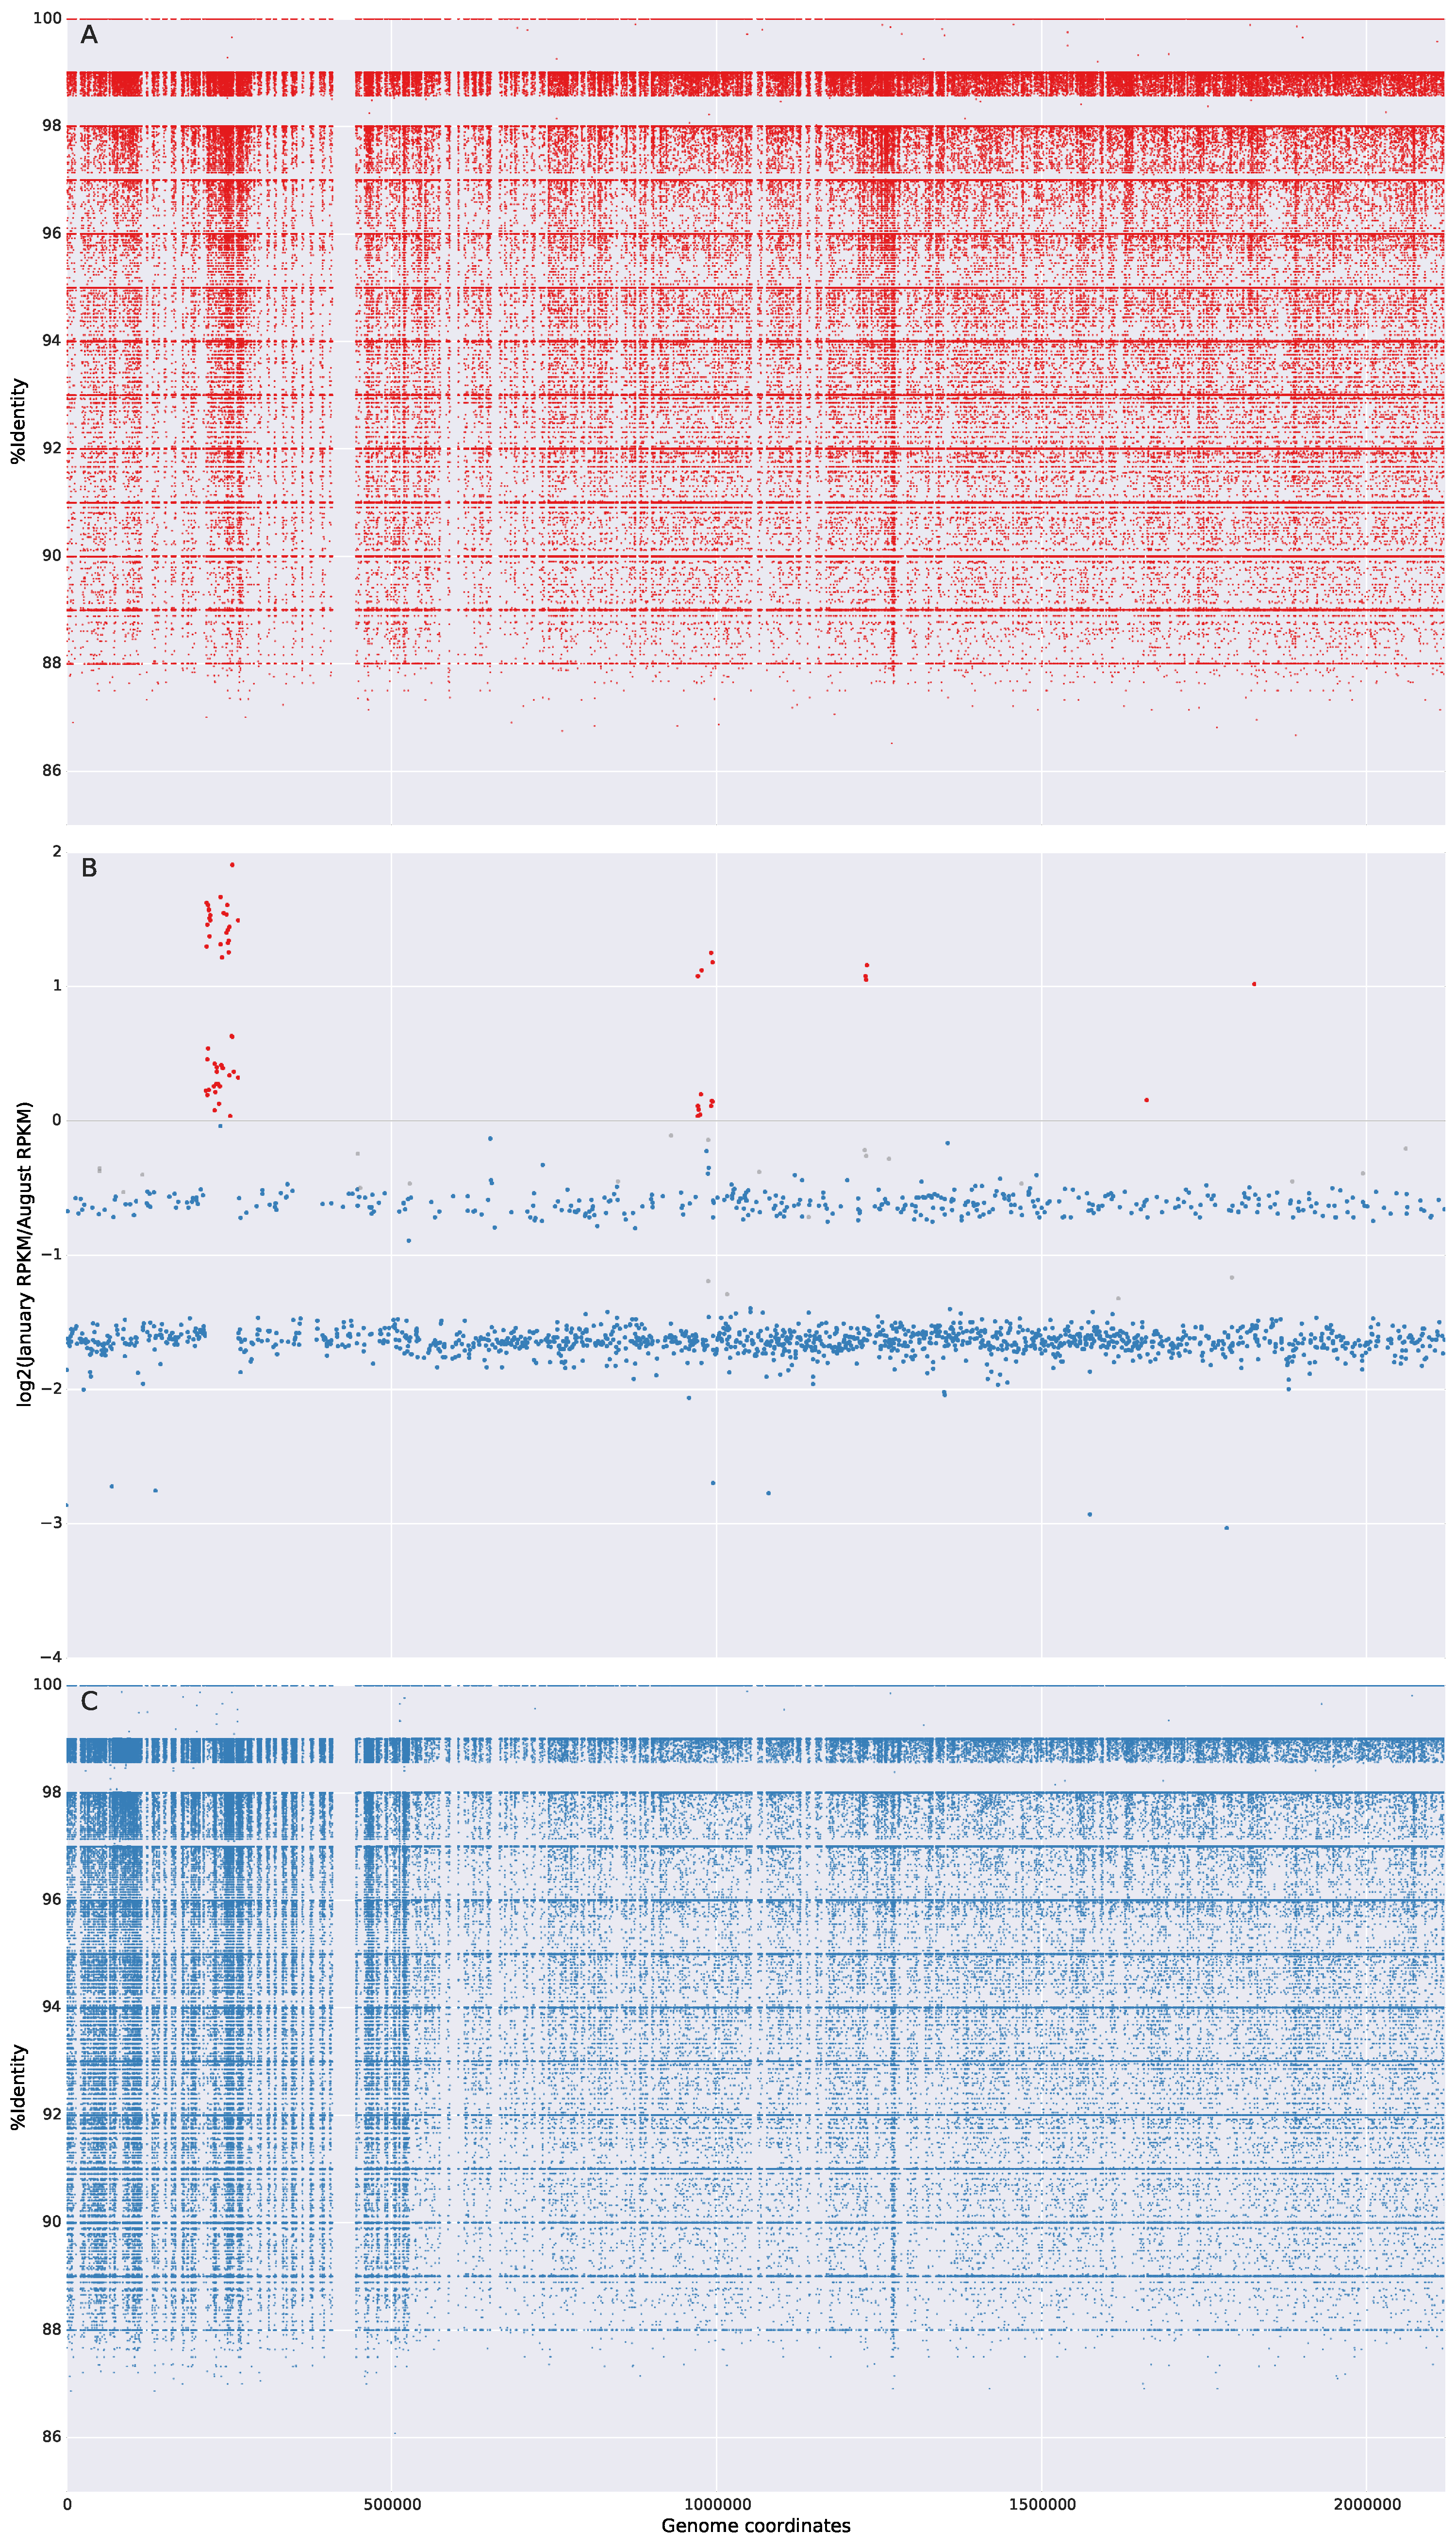
\includegraphics[width=\textwidth,height=\textheight,keepaspectratio]{Chapter5/Figures/coverage_plots/J07HR59_coverage.pdf}
  \caption{J07HR59coverage}
  \label{J07HR59coverage}
\end{figure}

\begin{figure}[!hbtp]
  \centering
  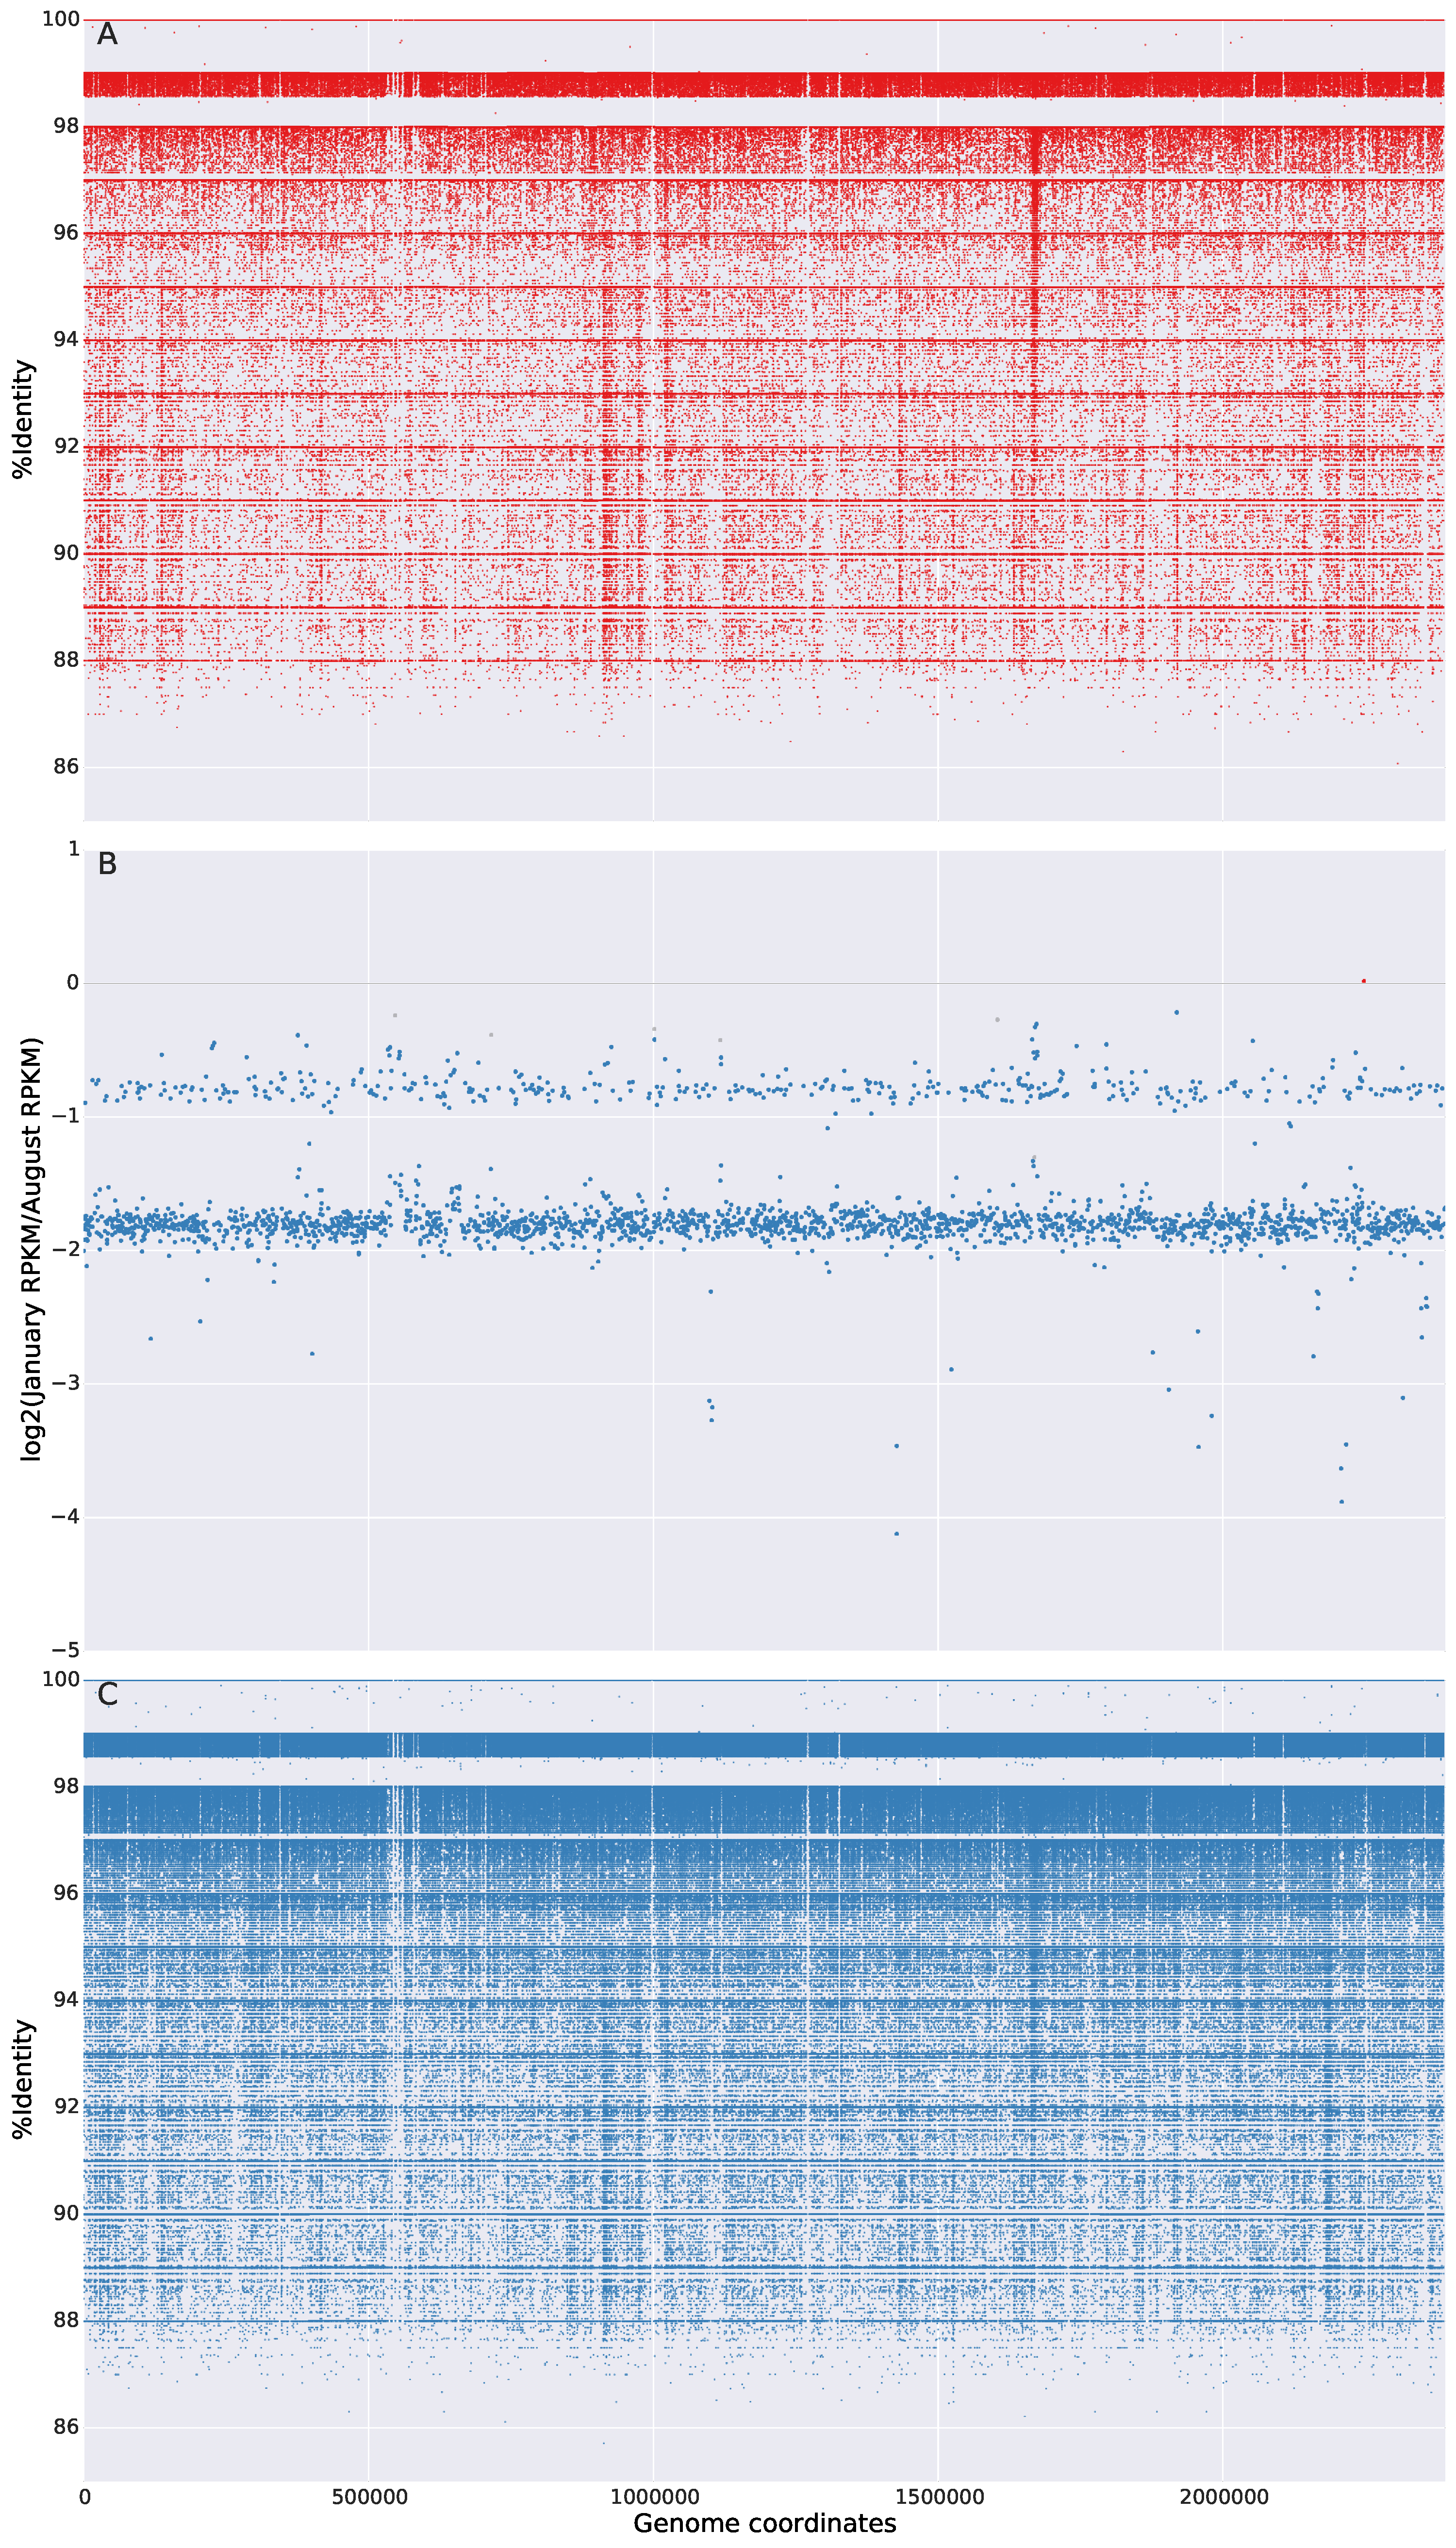
\includegraphics[width=\textwidth,height=\textheight,keepaspectratio]{Chapter5/Figures/coverage_plots/A07HB70_coverage.pdf}
  \caption{A07HB70coverage}
  \label{A07HB70coverage}
\end{figure}

\begin{figure}[!hbtp]
  \centering
  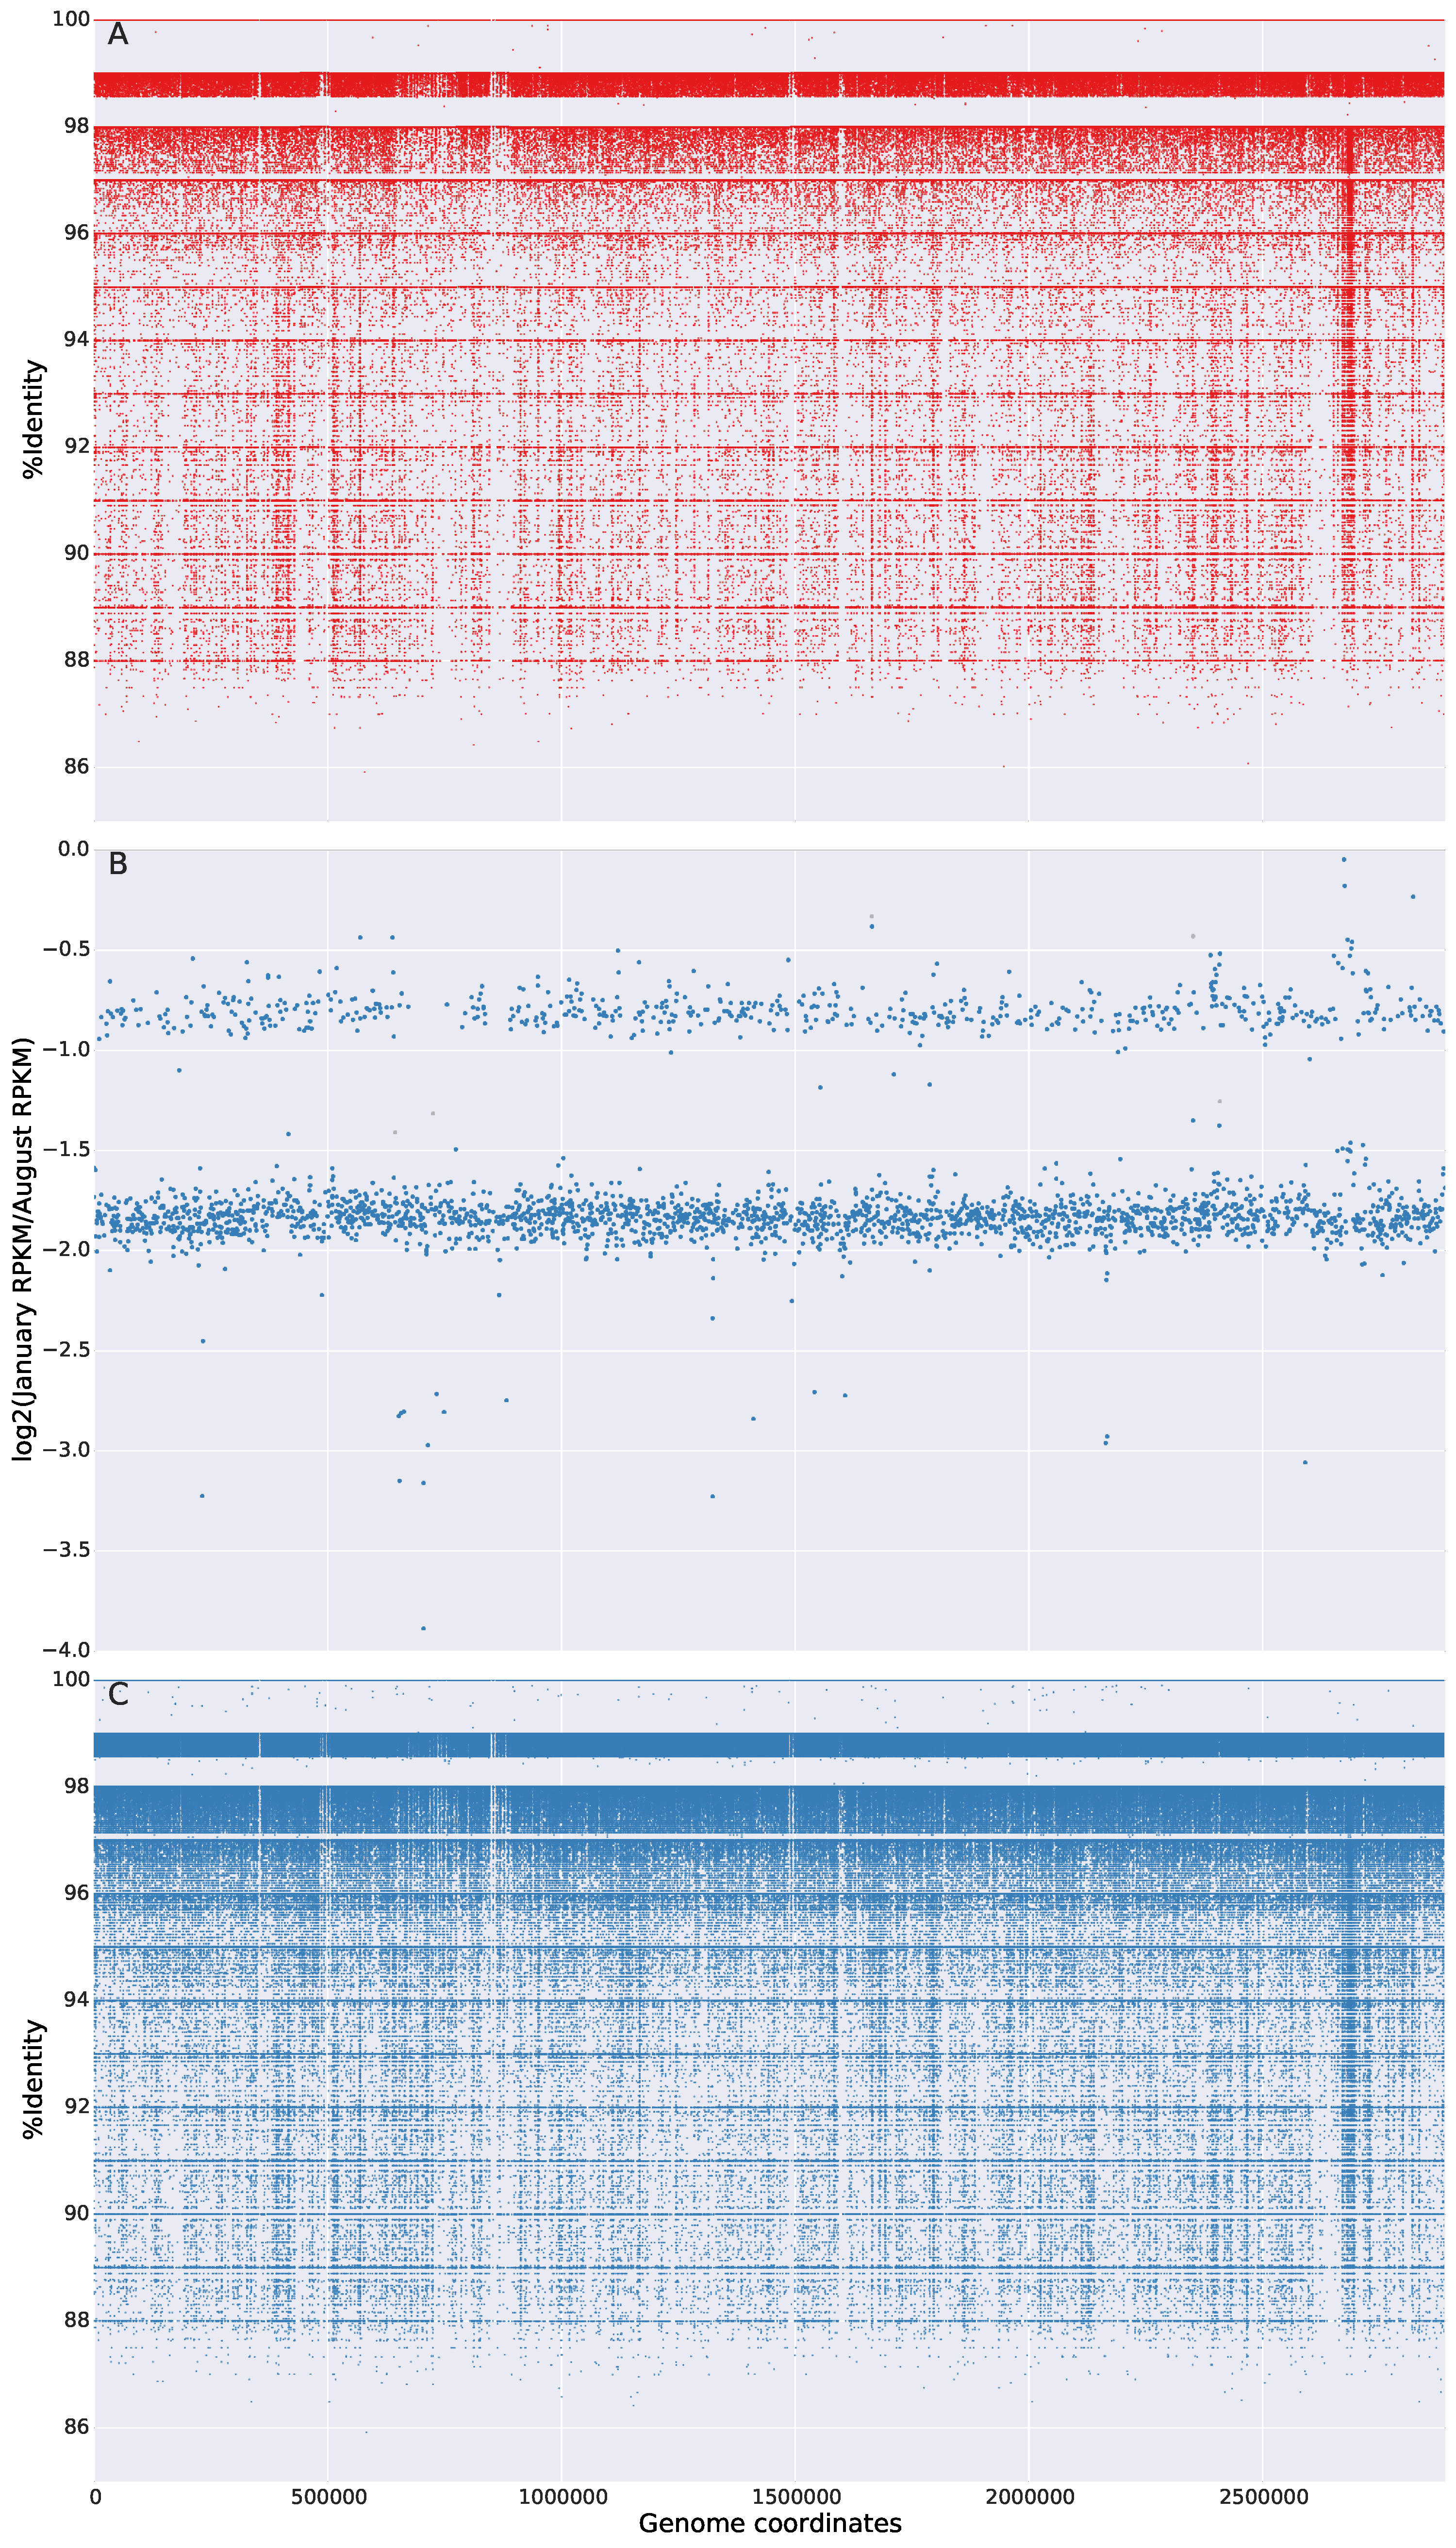
\includegraphics[width=\textwidth,height=\textheight,keepaspectratio]{Chapter5/Figures/coverage_plots/A07HR67_coverage.pdf}
  \caption{A07HR67coverage}
  \label{A07HR67coverage}
\end{figure}

\begin{figure}[!hbtp]
  \centering
  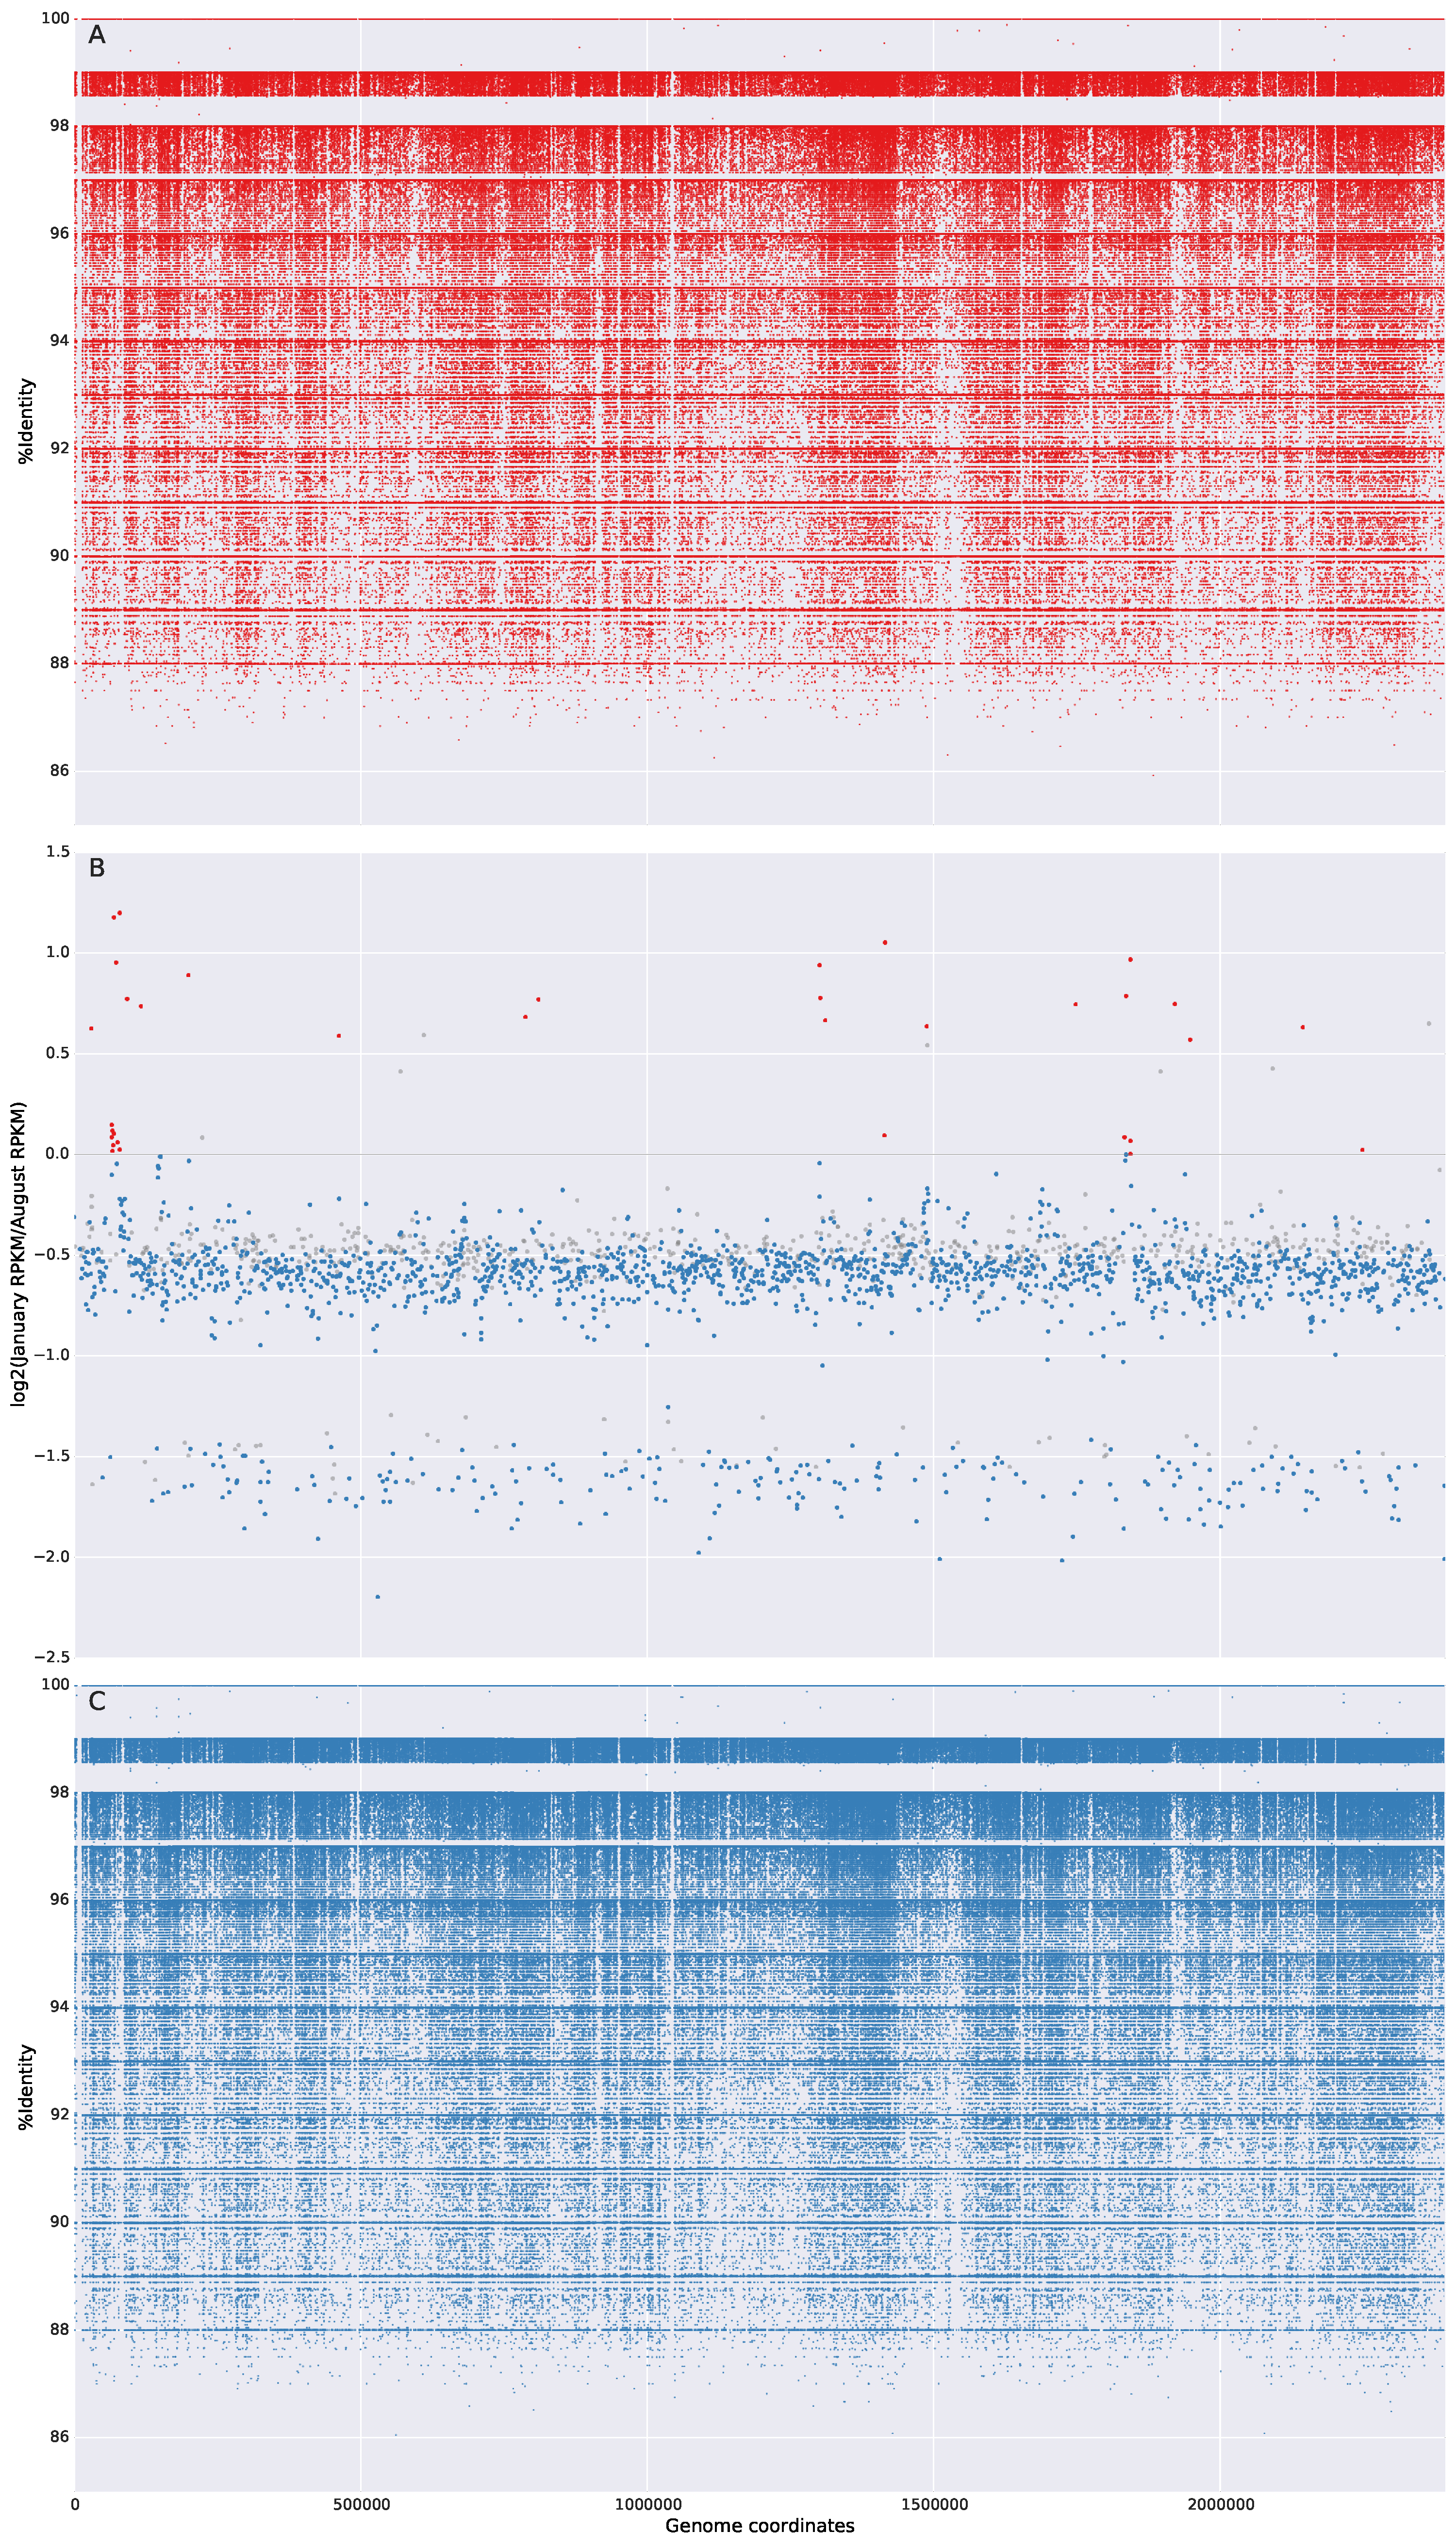
\includegraphics[width=\textwidth,height=\textheight,keepaspectratio]{Chapter5/Figures/coverage_plots/A07HN63_coverage.pdf}
  \caption{A07HN63coverage}
  \label{A07HN63coverage}
\end{figure}

\begin{figure}[!hbtp]
  \centering
  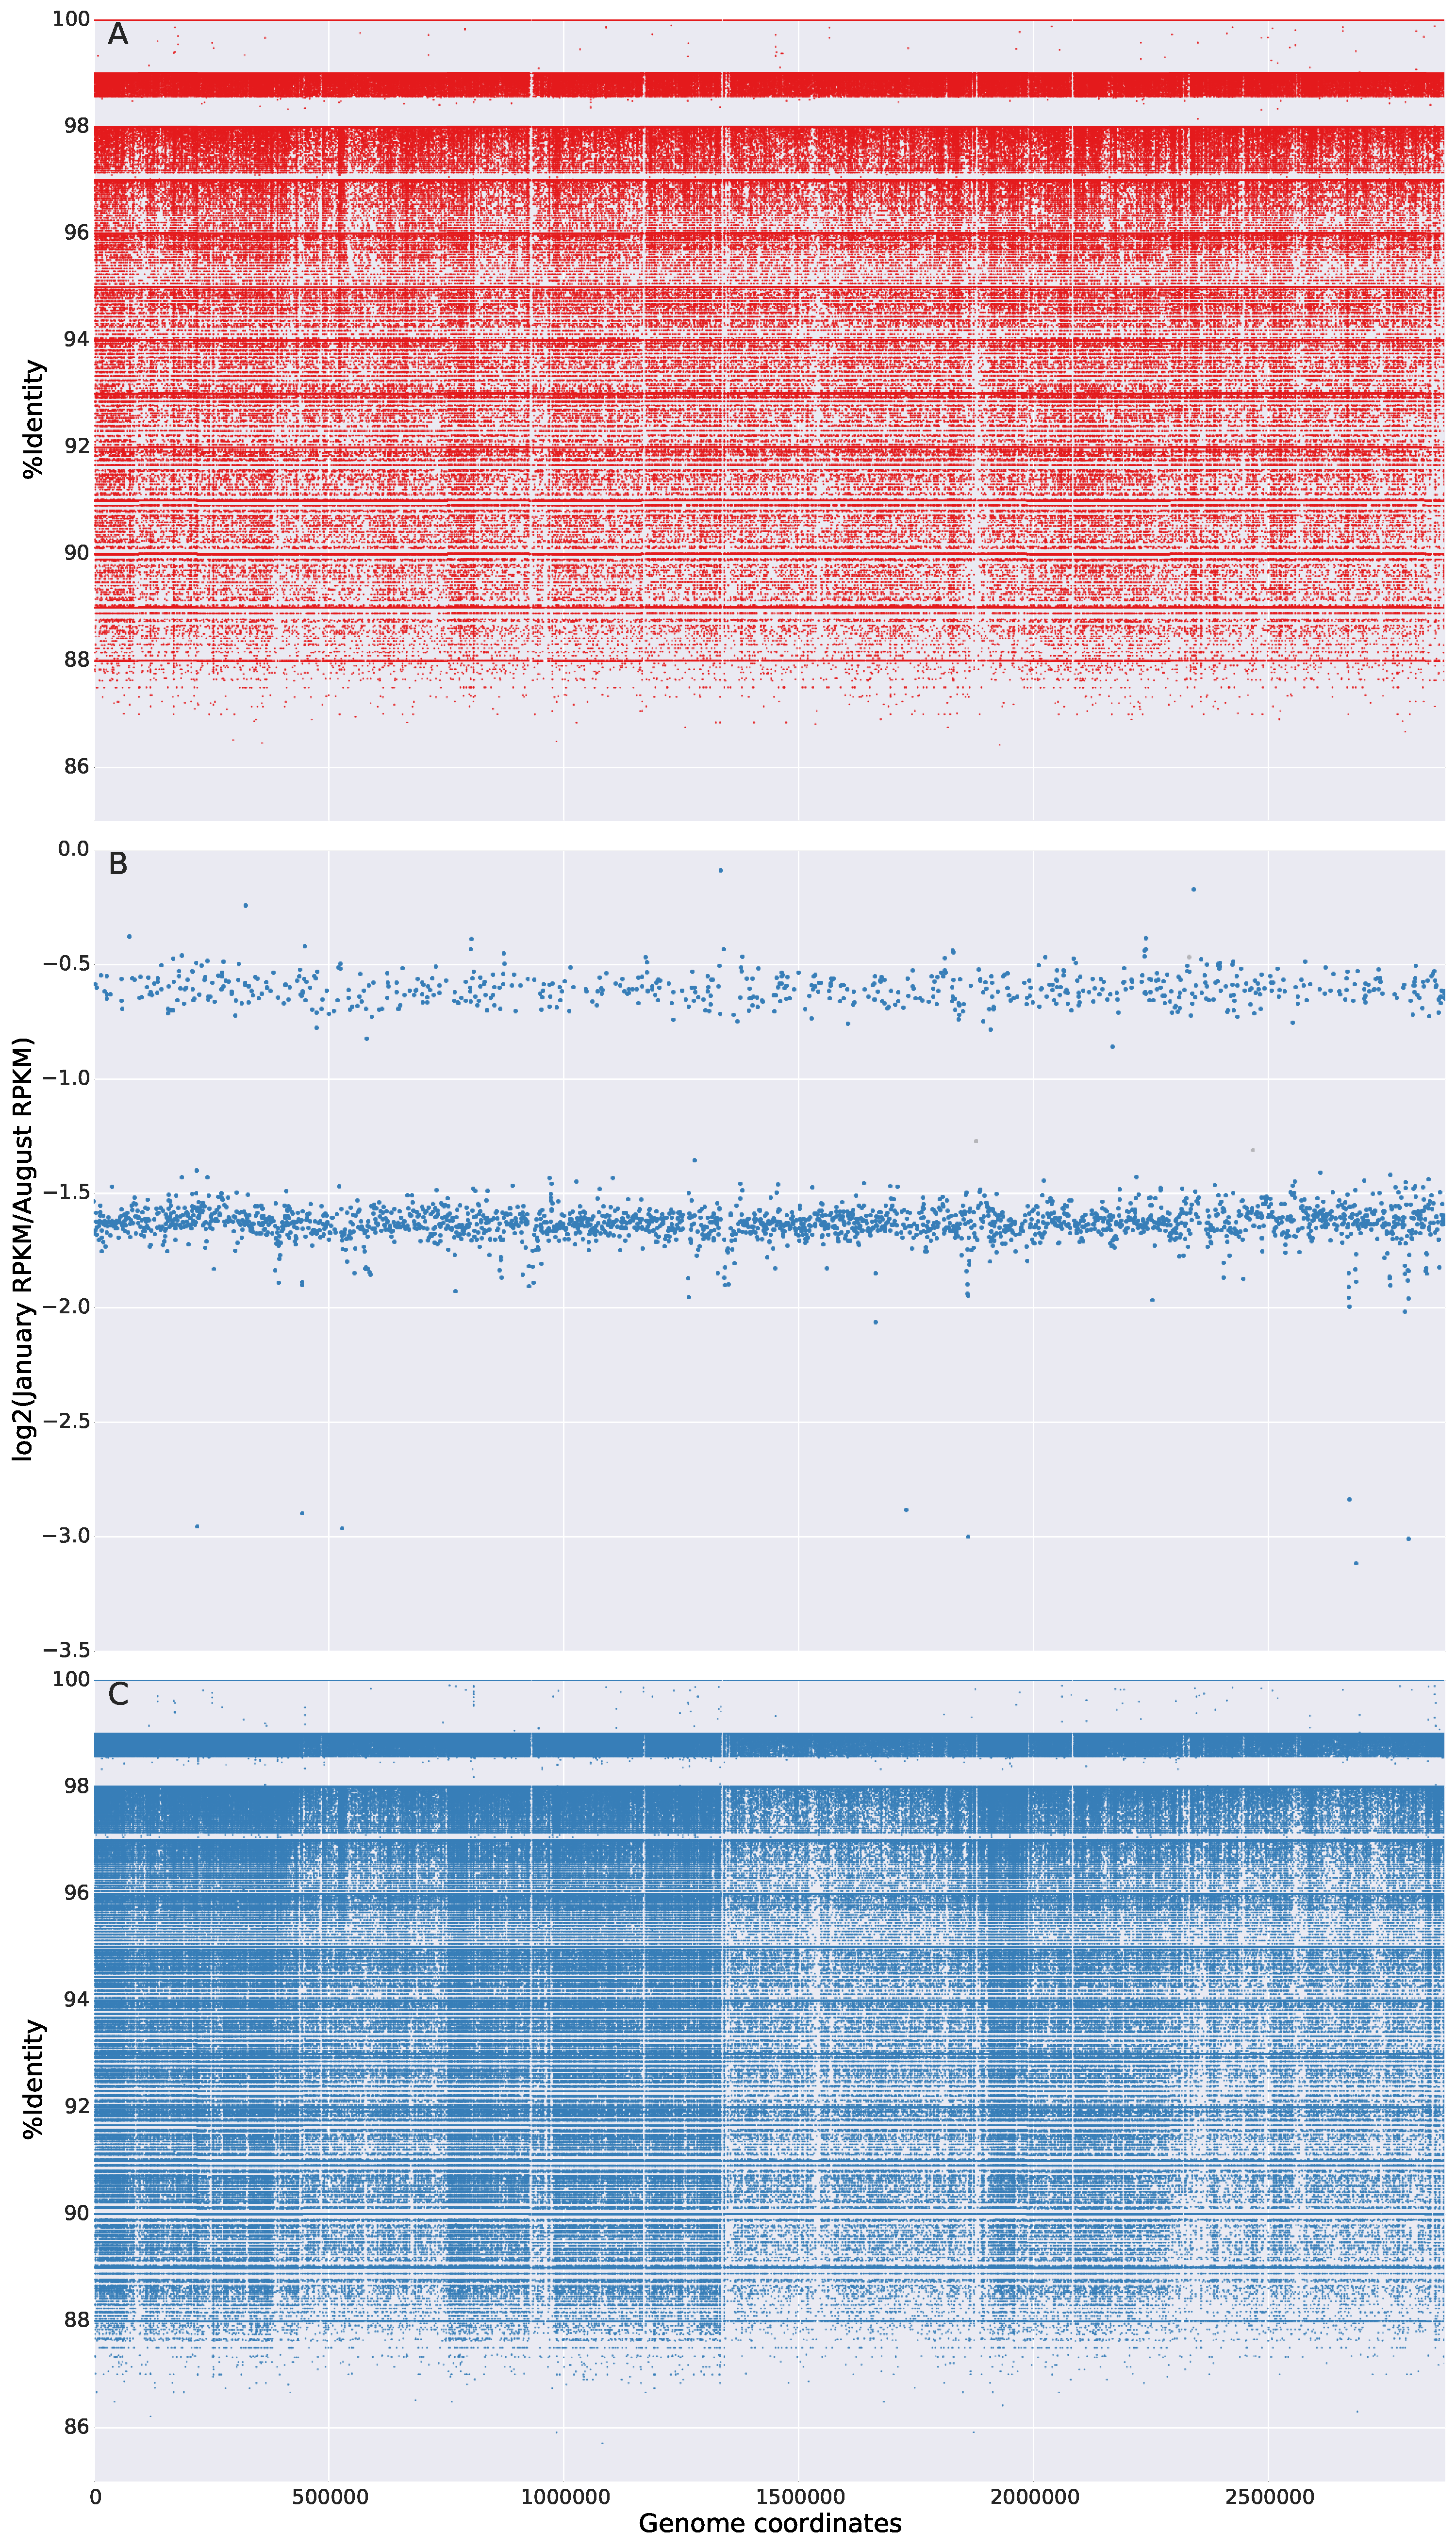
\includegraphics[width=\textwidth,height=\textheight,keepaspectratio]{Chapter5/Figures/coverage_plots/A07HR60_coverage.pdf}
  \caption{A07HR60coverage}
  \label{A07HR60coverage}
\end{figure}

\begin{figure}[!hbtp]
  \centering
  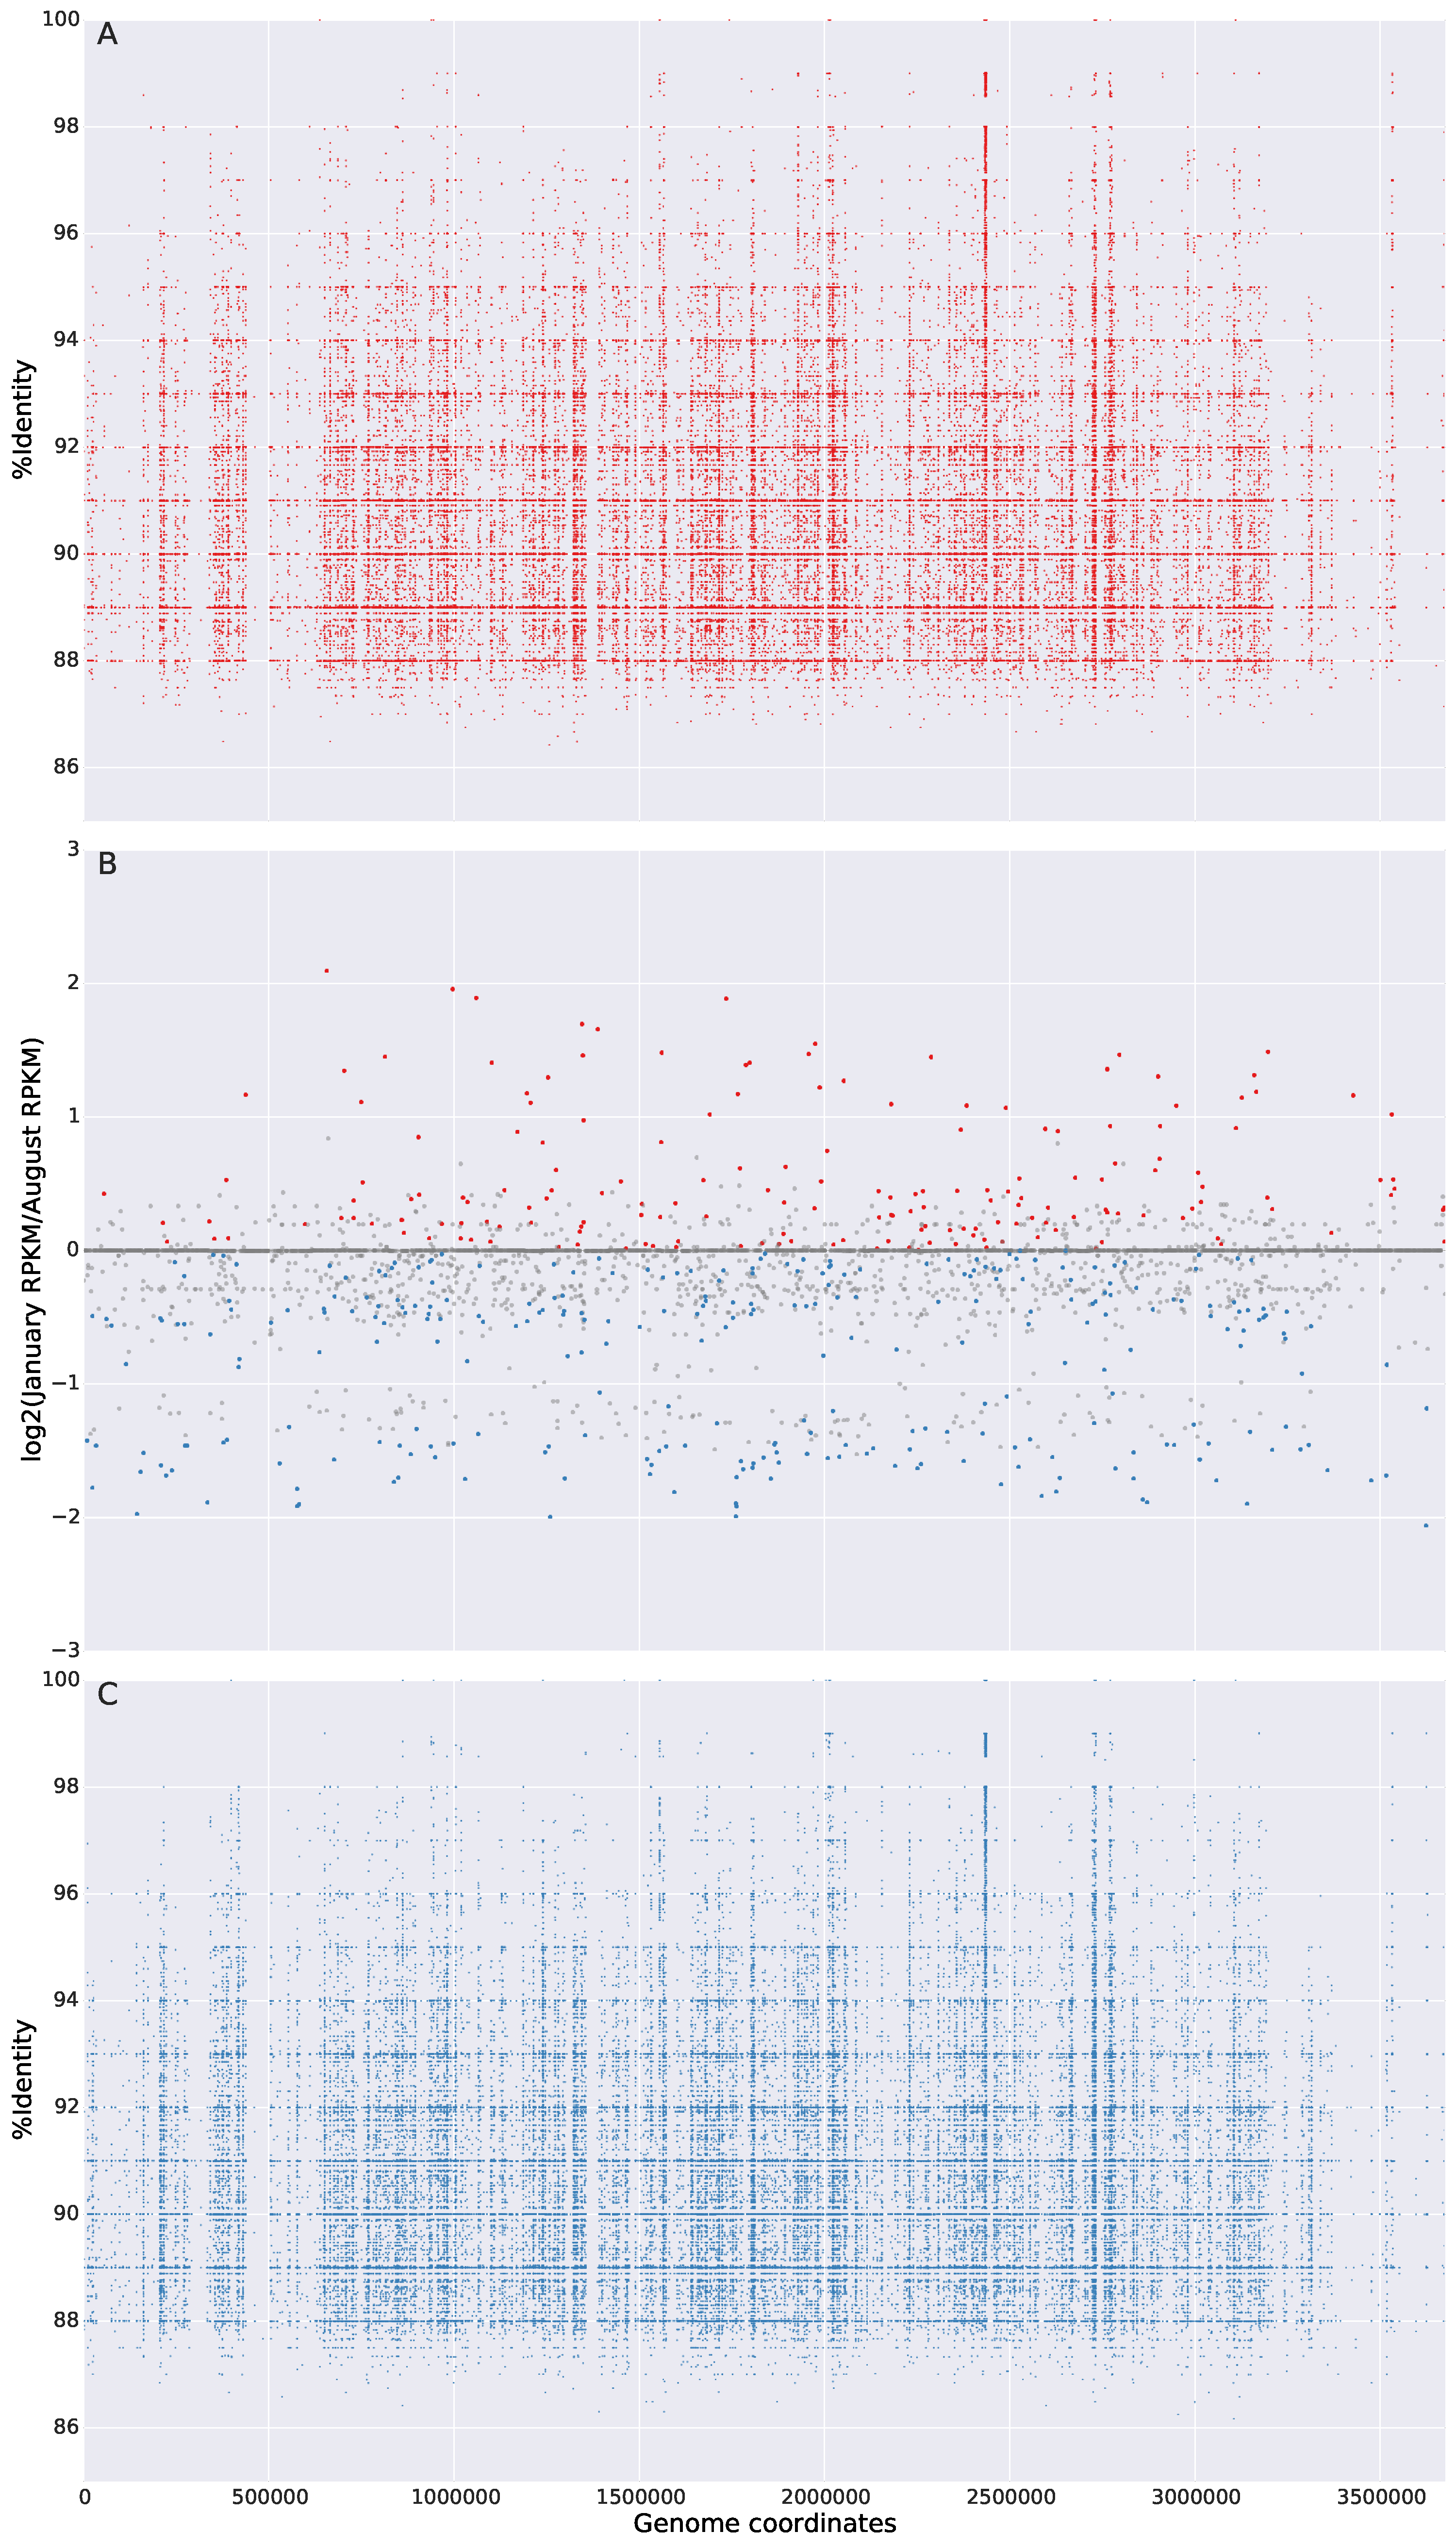
\includegraphics[width=\textwidth,height=\textheight,keepaspectratio]{Chapter5/Figures/coverage_plots/G22_coverage.pdf}
  \caption{G22 coverage}
  \label{G22coverage}
\end{figure}

\begin{figure}[!hbtp]
  \centering
  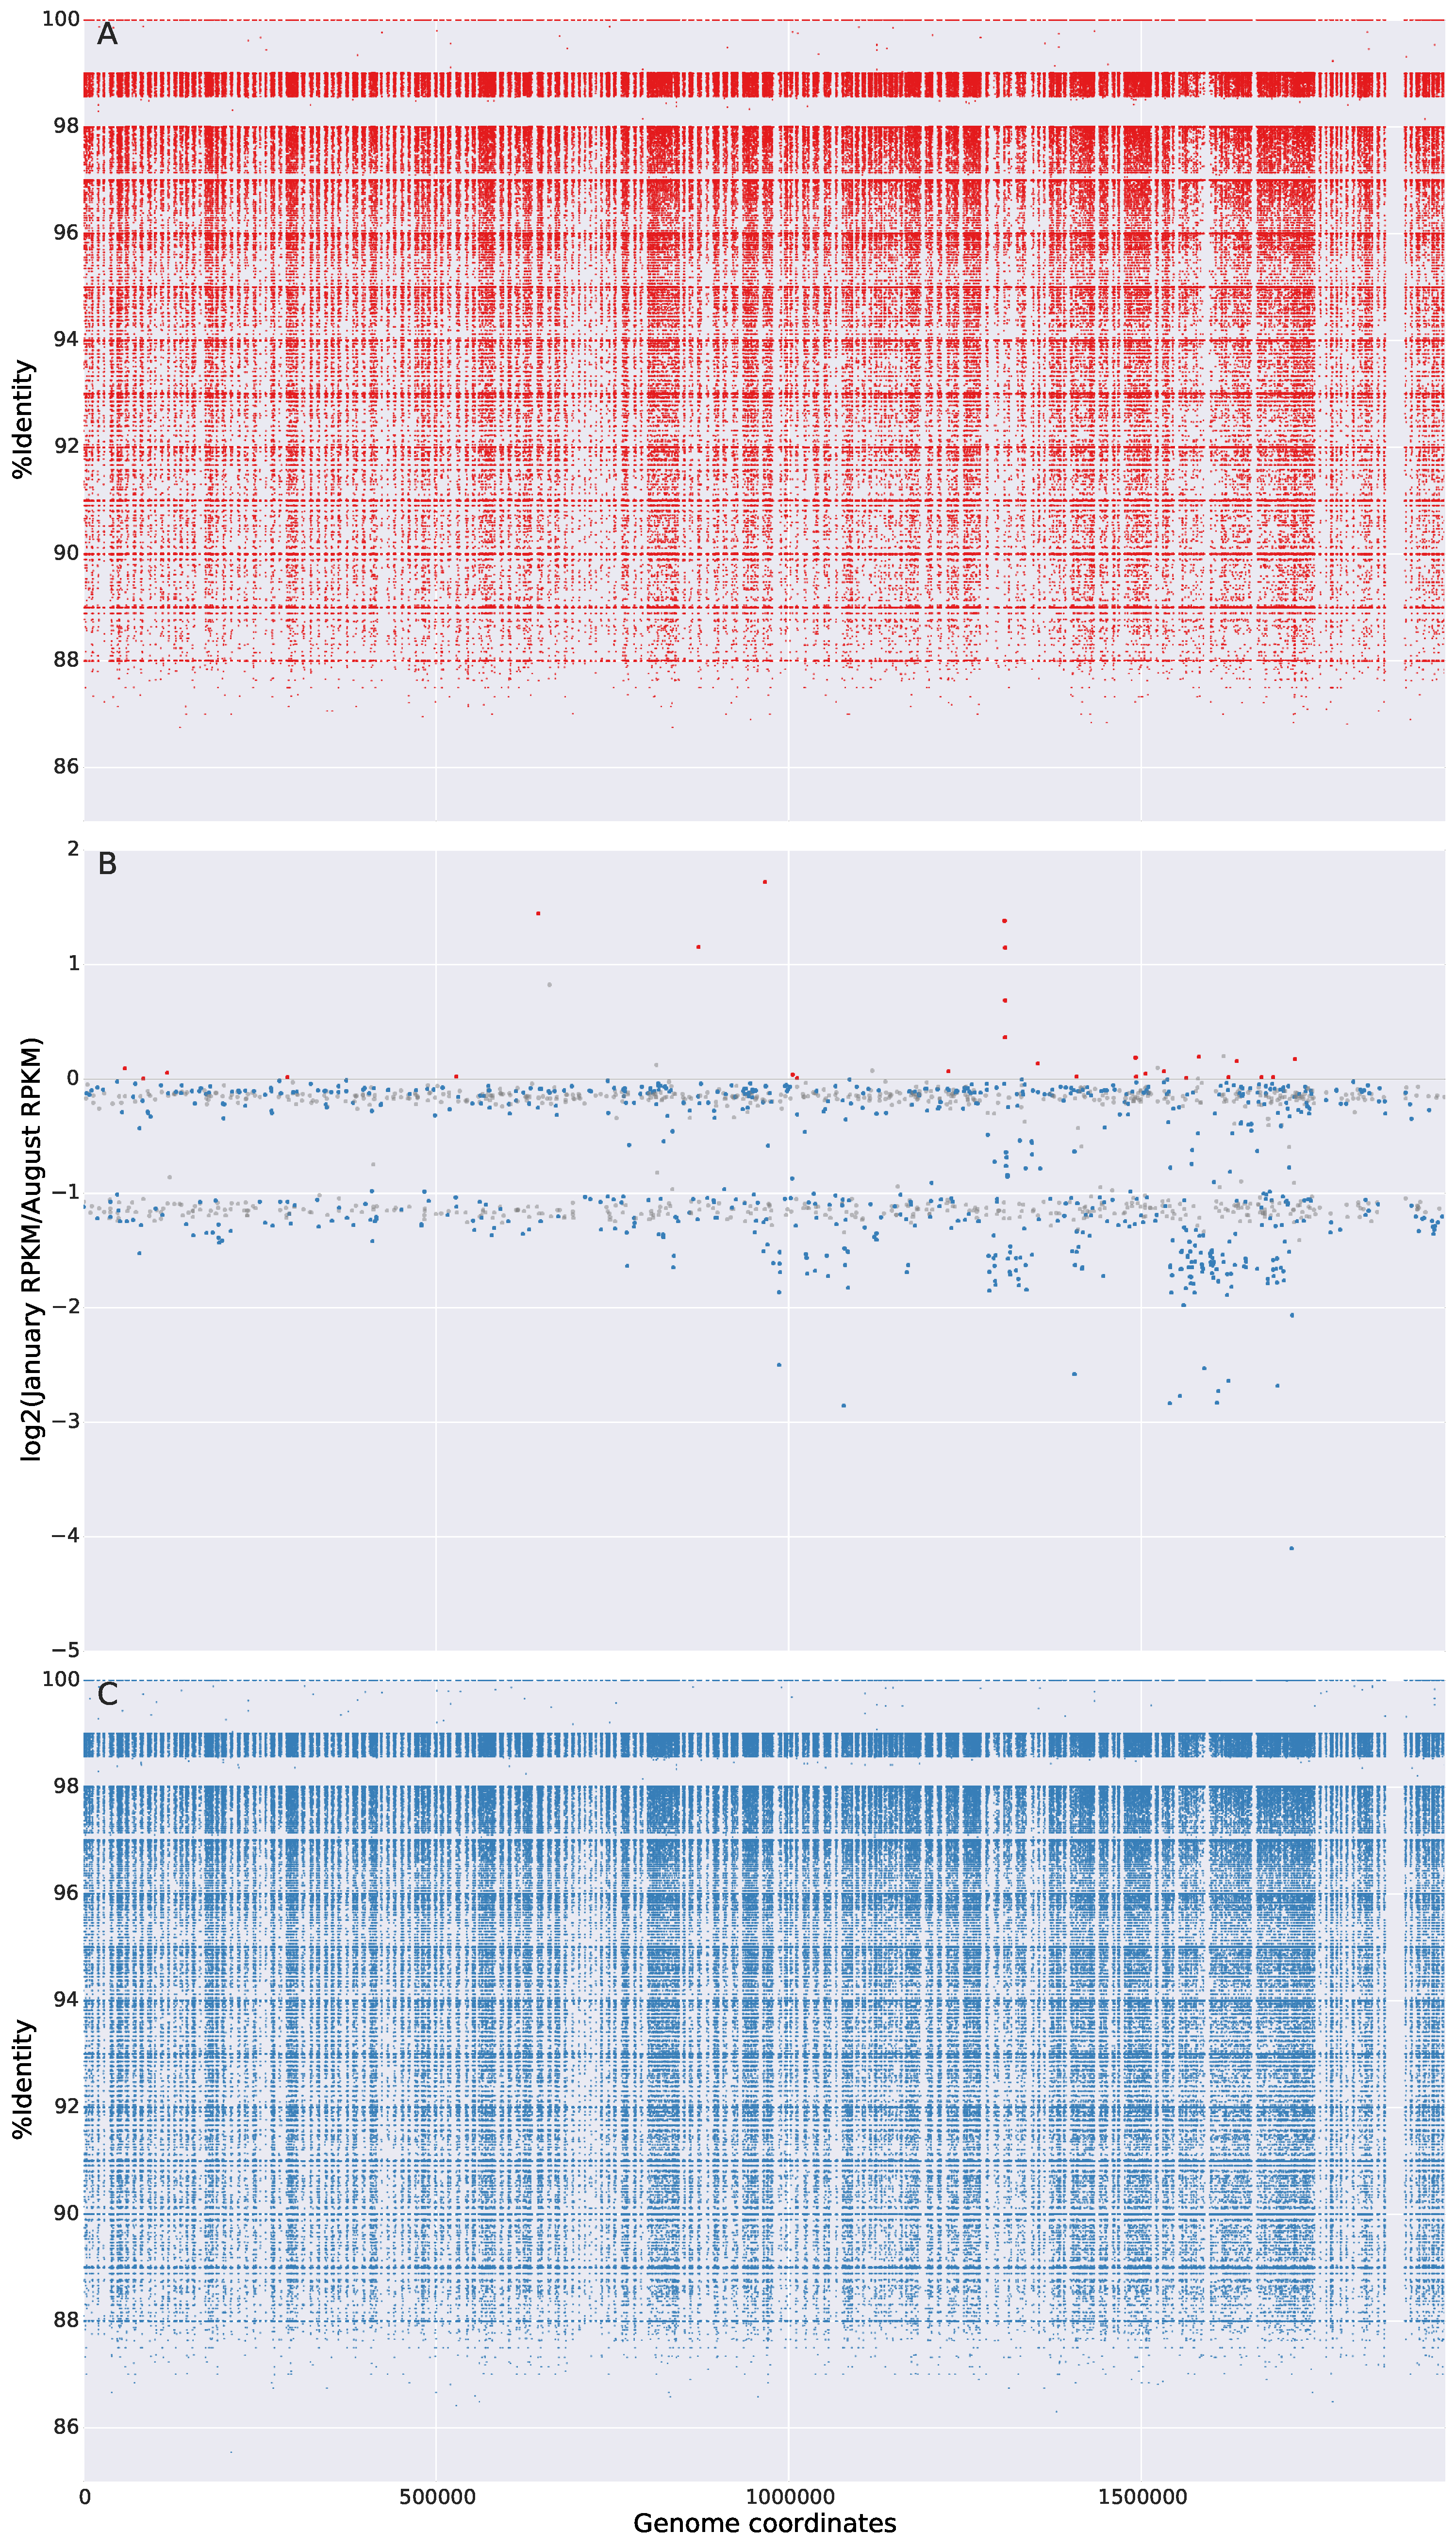
\includegraphics[width=\textwidth,height=\textheight,keepaspectratio]{Chapter5/Figures/coverage_plots/J07SB_coverage.pdf}
  \caption{J07SB coverage}
  \label{J07SBcoverage}
\end{figure}
